%%%%%%%%%%%%%%%%%%%%%%%%%%%%%%%%%%%%%%%%%%%%%%%%%%%%%%%%%%%%%%%%%%%%%%%%%%%%%%%%
% Univerzita Komenskeho - Thesis template
% Based on "Vnutorny predpis c. 12/2013"
%%%%%%%%%%%%%%%%%%%%%%%%%%%%%%%%%%%%%%%%%%%%%%%%%%%%%%%%%%%%%%%%%%%%%%%%%%%%%%%%

%%%%%%%%%%%%%%%%%%%%%%%%%%%%%%%%%%%%%%%%%%%%%%%%%%%%%%%%%%%%%%%%%%%%%%%%%%%%%%%%
% Global document settings
%%%%%%%%%%%%%%%%%%%%%%%%%%%%%%%%%%%%%%%%%%%%%%%%%%%%%%%%%%%%%%%%%%%%%%%%%%%%%%%%
% Cl.7/2 - font size 12pt, portrait, A4
% Cl.7/6 - single side printing
\documentclass[a4paper,12pt,oneside,final]{memoir}
% Cl.7/2 - 1.5x line spacing
\OnehalfSpacing

%%%%%%%%%%%%%%%%%%%%%%%%%%%%%%%%%%%%%%%%%%%%%%%%%%%%%%%%%%%%%%%%%%%%%%%%%%%%%%%%
% Page geometry
%%%%%%%%%%%%%%%%%%%%%%%%%%%%%%%%%%%%%%%%%%%%%%%%%%%%%%%%%%%%%%%%%%%%%%%%%%%%%%%%
\settypeblocksize{247mm}{155mm}{*}
% Cl.7/3 - 3.5cm left, 2cm right
% Cl.7/3 - 2.5cm top, 2.5cm bottom
\setlrmarginsandblock{3.5cm}{2cm}{*}
\setulmarginsandblock{2.5cm}{2.5cm}{*}
\checkandfixthelayout

%%%%%%%%%%%%%%%%%%%%%%%%%%%%%%%%%%%%%%%%%%%%%%%%%%%%%%%%%%%%%%%%%%%%%%%%%%%%%%%%
% Language, encoding, fonts
%%%%%%%%%%%%%%%%%%%%%%%%%%%%%%%%%%%%%%%%%%%%%%%%%%%%%%%%%%%%%%%%%%%%%%%%%%%%%%%%
% TODO pick fonts
%\usepackage{charter}


\usepackage{fontspec}
\usepackage{polyglossia}
\setdefaultlanguage{slovak}
%%%%%%%%%%%%%%%%%%%%%%%%%%%%%%%%%%%%%%%%%%%%%%%%%%%%%%%%%%%%%%%%%%%%%%%%%%%%%%%%
% Important packages
%%%%%%%%%%%%%%%%%%%%%%%%%%%%%%%%%%%%%%%%%%%%%%%%%%%%%%%%%%%%%%%%%%%%%%%%%%%%%%%%
\usepackage{microtype} % Typographical improvements
\usepackage{booktabs} % Better looking tables
\usepackage{pdfpages} % Include PDFs
\usepackage[bottom]{footmisc} % Move footnotes to the bottom

\usepackage[binary-units=true]{siunitx} % SI units + binary prefix (Mi, Gi, ...)
\usepackage{xspace} % Smart space for macros

% Figures
\newsubfloat{figure} % Allow subfigures
\usepackage{graphicx} % Images
\usepackage{threeparttable} % Tables
\usepackage{rotating} % Sideways figures

% TikZ illustrations
\usepackage{tikz}
\usepackage{tikz-qtree}
\usetikzlibrary{calc, fit}
\usetikzlibrary{patterns, shadings, shadows.blur}
\usetikzlibrary{decorations.pathmorphing,decorations.pathreplacing}
\usepgflibrary{decorations.markings}

% Modified from http://tex.stackexchange.com/a/17578/23342
% Center around any rect by redefining bounding box, can use node names
\tikzset{xcenter around/.style 2 args={execute at end picture={%
  \useasboundingbox let \p0 = (current bounding box.south west), \p1 = (current bounding box.north east),
                        \p2 = #1, \p3 = #2
                    in
        ({min(\x2 + \x3 - \x1,\x0)},\y0) rectangle ({max(\x3 + \x2 - \x0,\x1)},\y1);
}}}

\newcommand*{\FiguresPath}{figures}

% Math related
\usepackage{amsmath,amsthm}
\usepackage{amsfonts}
\usepackage{mathtools}
\usepackage{bm, mathrsfs}

% Custom symbols imported from fonts
% Import extra symbols

\DeclareFontFamily{U} {MnSymbolA}{}

\DeclareFontShape{U}{MnSymbolA}{m}{n}{
  <-6> MnSymbolA5
  <6-7> MnSymbolA6
  <7-8> MnSymbolA7
  <8-9> MnSymbolA8
  <9-10> MnSymbolA9
  <10-12> MnSymbolA10
  <12-> MnSymbolA12}{}
\DeclareFontShape{U}{MnSymbolA}{b}{n}{
  <-6> MnSymbolA-Bold5
  <6-7> MnSymbolA-Bold6
  <7-8> MnSymbolA-Bold7
  <8-9> MnSymbolA-Bold8
  <9-10> MnSymbolA-Bold9
  <10-12> MnSymbolA-Bold10
  <12-> MnSymbolA-Bold12}{}

\DeclareSymbolFont{MnSyA} {U} {MnSymbolA}{m}{n}

\DeclareMathSymbol{\rhookdownarrow}{\mathrel}{MnSyA}{59}

% TODO? remove amsfonts, use unicode-math
% TODO? but change the ugly fonts
%\usepackage[]{unicode-math}

% Algoritms / pseudo-code
\usepackage[chapter]{algorithm}
\makeatletter \renewcommand{\ALG@name}{Algoritmus}
\usepackage[noend]{algpseudocode} % No explicit "end function" line
\newcommand*\AlgLet[2]{\State #1 $\gets$ #2} % X <- Y assignment 

% Code syntax highlighting
\usepackage[chapter]{minted}
\usemintedstyle{tango}
\renewcommand\listingscaption{Zdrojový kód}

%%%%%%%%%%%%%%%%%%%%%%%%%%%%%%%%%%%%%%%%%%%%%%%%%%%%%%%%%%%%%%%%%%%%%%%%%%%%%%%%
% Bibliography
%%%%%%%%%%%%%%%%%%%%%%%%%%%%%%%%%%%%%%%%%%%%%%%%%%%%%%%%%%%%%%%%%%%%%%%%%%%%%%%%
% TODO bibliography list layout
% TODO initials+2digit year?
%\usepackage[authoryear,square,sort]{natbib}
\usepackage[numbers,square,sort]{natbib}
\bibliographystyle{natdin}
% TODO language? "... in ..." -> "v"

%%%%%%%%%%%%%%%%%%%%%%%%%%%%%%%%%%%%%%%%%%%%%%%%%%%%%%%%%%%%%%%%%%%%%%%%%%%%%%%%
% Misc packages
%%%%%%%%%%%%%%%%%%%%%%%%%%%%%%%%%%%%%%%%%%%%%%%%%%%%%%%%%%%%%%%%%%%%%%%%%%%%%%%%
\usepackage{lipsum} % Lorem ipsum (for testing)

%\usepackage[color=white]{todonotes} % print mode
\usepackage{todonotes}

% XeLaTeX and BibTex
\usepackage{metalogo}
\usepackage{dtklogos}

\usepackage{ccicons}

%%%%%%%%%%%%%%%%%%%%%%%%%%%%%%%%%%%%%%%%%%%%%%%%%%%%%%%%%%%%%%%%%%%%%%%%%%%%%%%%
% Setup document preferences
%%%%%%%%%%%%%%%%%%%%%%%%%%%%%%%%%%%%%%%%%%%%%%%%%%%%%%%%%%%%%%%%%%%%%%%%%%%%%%%%
% Chapter style
\makeatletter

\newlength{\numberheight}
\setlength{\numberheight}{\beforechapskip}

\newlength{\barlength}
\newlength{\chnumwidth}

\newlength{\namenumsep}
\setlength{\namenumsep}{0.5em}

\newlength{\numbarsep}
\setlength{\numbarsep}{1em}

% Modified from 'veelo' style in memoir and
% https://tex.stackexchange.com/questions/69656/right-align-chapter-number-to-the-chapter-name-when-using-memoir-with-veelo-styl

\makechapterstyle{myveelo}{%
    \setlength{\afterchapskip}{40pt}
    \renewcommand*{\chapterheadstart}{\vspace*{40pt}}
    \renewcommand*{\afterchapternum}{\par\nobreak\vskip 25pt}
    \renewcommand*{\chapnamefont}{\normalfont\LARGE\flushright}
    \renewcommand*{\chapnumfont}{\normalfont\HUGE}
    \renewcommand*{\chaptitlefont}{\normalfont\HUGE\bfseries\flushright}
    \renewcommand*{\chapternamenum}{}
    
    \setlength{\midchapskip}{\paperwidth}
    \addtolength{\midchapskip}{-\textwidth}
    \addtolength{\midchapskip}{-\spinemargin}
    
    \setlength{\barlength}{\midchapskip}
    \addtolength{\barlength}{-\numbarsep}
        
    \renewcommand*{\printchaptername}{%
        \settowidth{\chnumwidth}{\resizebox{!}{\numberheight}{\chapnumfont \thechapter}}%
        \chapnamefont\MakeUppercase{\@chapapp}%
        \hspace*{\chnumwidth}%
        \hspace*{\namenumsep}%
    }
    
    \renewcommand*{\printchapternum}{%
        \makebox[0pt][l]{
            \settowidth{\chnumwidth}{\resizebox{!}{\numberheight}{\chapnumfont \thechapter}}%
            \hspace*{-\chnumwidth}%
            \resizebox{!}{\numberheight}{\chapnumfont \thechapter}%
            \hspace*{\numbarsep}%
            \rule{\barlength}{\numberheight}%
    }}%
}

\makeatother
\chapterstyle{myveelo} % TODO pick - veelo, madsen, ?

% Subsections and higher - numbered and in TOC
\setsecnumdepth{subsection}
\maxtocdepth{subsection}

% Headers / footers
\pagestyle{ruled}
% https://tex.stackexchange.com/questions/176472/identical-marks-in-header-with-onesided-memoir/176484?noredirect=1#176484
% https://tex.stackexchange.com/questions/59565/on-testing-two-fully-expanded-character-strings-for-equality
\usepackage{pdftexcmds} 
\makeatletter
\newcommand*{\test}[2]{%
  \ifnum\pdf@strcmp{#1}{#2}=\z@ \relax \else #2 \fi
}
\makeatother
\makeoddhead{ruled}{\sffamily\leftmark}{}{\sffamily\test{\leftmark}{\rightmark}}

% Create custom plain page style with pagenumbers on right instead of centered
\makepagestyle{plainright}
\makeoddfoot{plainright}{}{}{\thepage}
\aliaspagestyle{chapter}{plainright}

% Custom caption rules
\newfixedcaption{\figcaption}{figure}
\newfixedcaption{\algcaption}{algorithm}

% Custom theorem enviroments
\newtheorem{theorem}{Theorem}[section]
\newtheorem{lema}[theorem]{Lema}

%%%%%%%%%%%%%%%%%%%%%%%%%%%%%%%%%%%%%%%%%%%%%%%%%%%%%%%%%%%%%%%%%%%%%%%%%%%%%%%%
% Macros
%%%%%%%%%%%%%%%%%%%%%%%%%%%%%%%%%%%%%%%%%%%%%%%%%%%%%%%%%%%%%%%%%%%%%%%%%%%%%%%%
\newcommand{\unnumberedchapter}[1]{
    \chapter*[#1]{#1}
    \addcontentsline{toc}{chapter}{#1}
}

% Generic shortcuts
\newcommand{\bigO}[1]{\ensuremath{\mathcal{O}(#1)}}
\newcommand{\inlcode}[1]{\texttt{#1}\xspace}

% Shortcuts specific to this document
\newcommand{\cache}{\emph{cache}\xspace}
\newcommand{\Cache}{\emph{Cache}\xspace}
\newcommand{\disk}{\emph{disk}\xspace}
\newcommand{\aware}{\emph{cache-aware}\xspace}
\newcommand{\Aware}{\emph{Cache-aware}\xspace}
\newcommand{\obliv}{\emph{cache-oblivious}\xspace}
\newcommand{\extmem}{\emph{external-memory}\xspace}
\newcommand{\RAM}{\emph{RAM model}\xspace}
\newcommand{\vEB}{\emph{van Emde Boas}\xspace}
\newcommand{\hit}{\emph{cache hit}\xspace}
\newcommand{\miss}{\emph{cache miss}\xspace}

%%%%%%%%%%%%%%%%%%%%%%%%%%%%%%%%%%%%%%%%%%%%%%%%%%%%%%%%%%%%%%%%%%%%%%%%%%%%%%%%
% Include document settings (title, name, ...)
%%%%%%%%%%%%%%%%%%%%%%%%%%%%%%%%%%%%%%%%%%%%%%%%%%%%%%%%%%%%%%%%%%%%%%%%%%%%%%%%
\def \settingsSchool{Univerzita Komenského v Bratislave}
\def \settingsFaculty{Fakulta matematiky, fyziky a informatiky}

\def \settingsTitle{Cache-oblivious algoritmy a ich vizualizácia}
\def \settingsAuthor{Ladislav Pápay}
\def \settingsYear{2014}

\def \settingsProgramme{Informatika}
\def \settingsField{2508?? Informatika} % TODO: cislo odboru
\def \settingsDepartment{Katedra Informatiky FMFI}
\def \settingsAdvisor{Mgr. Jakub Kováč, PhD.}

\def \settingsAISfile{ais-zadanie-export.pdf}

%%%%%%%%%%%%%%%%%%%%%%%%%%%%%%%%%%%%%%%%%%%%%%%%%%%%%%%%%%%%%%%%%%%%%%%%%%%%%%%%
% Hyperref setup
%%%%%%%%%%%%%%%%%%%%%%%%%%%%%%%%%%%%%%%%%%%%%%%%%%%%%%%%%%%%%%%%%%%%%%%%%%%%%%%%
\usepackage[hidelinks]{hyperref}
\hypersetup{
    unicode=true,
    pdftitle={\settingsTitle},
    pdfauthor={\settingsAuthor},
    bookmarksnumbered=true,     
    bookmarksopen=true,         
    bookmarksopenlevel=1,       
    pdfpagemode=UseOutlines
}

%%%%%%%%%%%%%%%%%%%%%%%%%%%%%%%%%%%%%%%%%%%%%%%%%%%%%%%%%%%%%%%%%%%%%%%%%%%%%%%%
% Start of document
%%%%%%%%%%%%%%%%%%%%%%%%%%%%%%%%%%%%%%%%%%%%%%%%%%%%%%%%%%%%%%%%%%%%%%%%%%%%%%%%
\begin{document}
\frontmatter
    \newcommand{\coverTop}{
    \begin{center}
        {\textbf \Large \textsc {\settingsSchool \\ \settingsFaculty}}
        \vfill
        {\LARGE \em \settingsTitle}
        \\
        \medskip
        {\large Bakalárska práca}
    \end{center}
}

\newcommand{\coverCenter}{
    \begin{tabular}{l l}
        \textbf{Študijný program:} & \settingsProgramme \\
        \textbf{Študijný odbor:} & \settingsField \\
        \textbf{Školiace pracovisko:} & \settingsDepartment \\
        \textbf{Vedúci práce:} &  \settingsAdvisor
    \end{tabular}
}

\newcommand{\coverBottom}{
    \begin{center}
        \textbf{\settingsYear \hfill \settingsAuthor}
    \end{center}
}

\thispagestyle{empty}
\coverTop
\vfill
\coverBottom
\newpage

\thispagestyle{empty}
\coverTop
\vfill
\coverCenter
\vfill
\coverBottom
\newpage



    \includepdf[pages=1]{\settingsAISfile}
    \newpage
    
    \thispagestyle{plainright}
    ~\vfill
\section*{Poďakovanie}

Za návrh témy a odbornú pomoc pri jej spracovaní patrí vďaka môjmu školiteľovi Jakubovi Kováčovi. Ďalej ďakujem svojim priateľom za testovanie a spätnú väzbu počas spracúvania tejto práce. V neposlednom rade ďakujem rodine za podporu a poskytnuté možnosti vzdelávania.

\vspace{3cm}

    \newpage
    
    \chapter*{Abstrakt}

V tejto práci sa zaoberáme modelmi externej pamäte, ktoré vystihujú hierarchické pamäte v dnešných výpočtových systémoch. Konkrétne uvádzame takzvaný \emph{cache-oblivious model} model, ktorý pre isté problémy dosahuje optimálne výsledky bez znalosti parametrov tejto pamäťovej hierarchie. Pre tento model uvádzame niekoľko algoritmov a dátových štruktúr, hlavne B-stromy, spolu s analýzou počtu pamäťových presunov. Napokon v poslednej časti práce popisujeme funkcionalitu a používanie vizualizácií vytvorených ako súčasť tejto práce.

Výsledkom práce sú vizualizácie pre niekoľko vybraných \obliv dátových štruktúr, ktoré sú implementované ako rozšírenie aplikácie \emph{Gnarley Trees}, ktorá vznikla ako súčasť bakalárskej práce Jakuba Kováča v roku 2007. Na priloženom CD sa nachádza zdrojový kód a spustiteľná verzia tejto aplikácie.


\vspace{2cm}
\noindent\textsc{Kľúčové slová:} dátové štruktúry, pamäťová analýza, cache, cache-oblivious, vizualizácia

\newpage
\chapter*{Abstract}
In this thesis we consider models of external memory, which capture the hierarchical memory used in today's computer systems. In particular we describe the so called \emph{cache-oblivious model} which for some problems achieves optimal results without the need to know the parameters of this memory hierarchy. We describe several algorithms and data structures in this model, primarily B-trees, together with analysis of their memory transfers. In the last part we describe the features and usage of visualizations created as a part of this work.

The result of this thesis is visualization of several selected \obliv data structures implemented as an extension of the \emph{Gnarley Trees} application, which was created as a part of bachelor's thesis by Jakub Kováč in 2007. The attached CD contains source code and executable version of this application. 

\vspace{2cm}
\noindent\textsc{Keywords:} data structures, memory analysis, cache, cache-oblivious, visualizations
    \newpage
    
    \tableofcontents*
    \newpage
    \listoffigures*
    \newpage
    \listoftables*
    
\mainmatter
    \unnumberedchapter{Úvod}
% TODO epigraph?

Pri tvorbe efektívnych algoritmov sa najčastejšie zaujímame o časovú zložitosť a prípadne aj pamäťovú zložitosť. Dôležitým faktorom však môže byť aj množstvo pamäťových operácií. Tie majú priamy vplyv na výslednú časovú zložitosť avšak pri asymptotickej analýze sa často považujú za operáciu vykonateľnú v konštantnom čase. V prípadoch keď pracujeme s veľkým objemom dát, ktoré sú uložené na médiu s veľkou kapacitou ale nízkou prístupovou rýchlosťou, môže byť výhodné minimalizovať množstvo zápisov a čítaní z tohto média.

Klasickým prístupom v týchto prípadoch boli takzvané \aware algoritmy, ktoré potrebujú poznať presné parametre pamäťového systému pre dosiahnutie požadovanej efektivity. V tejto práci sa budeme venovať \obliv algoritmom, ktoré sú asymptoticky rovnako efektívne ako \aware, avšak bez nutnosti poznať parametre pamäte.

Okrem samozrejmej výhody, kedy nám stačí jedna univerzálna implementácia algoritmu pre ľubovolné množstvo rôznych systémov, prinášajú tieto algoritmy aj iné zlepšenia. V takmer každom systéme je pamäť hierarchická, zložená z viacerých úrovní, pričom každá je väčšia ale pomalšia ako predošlá. Pri \aware by pre optimálne využitie každej z úrovní pamäte bolo potrebné poznať parametre každej úrovne, a rekurzívne vnoriť do seba mnoho inštancií, každú optimalizovanú pre jednu úroveň. No v \obliv nám stačí jedna inštancia - keďže nepozná parametre žiadnej úrovne, bude rovnako dobre fungovať na každej z nich.

Súčasťou práce je vysvetliť problematiku \obliv pamäťového modelu, uviesť prehlad algoritmov a dátových štruktúr a vytvoriť vizualizácie vybraných z nich. Vizualizácie sú implementované ako súčasť programu {\em Alg-Vis}. Cieľom týchto vizualizácií je umožniť užívateľom experimentovať s implementáciou týchto algoritmov a dátových štruktúr, sledovať ich prácu krok po kroku a uľahčiť ich porozumeniu.a
\chapter{Pamäťový model}
\epigraph{Memory is the thing you forget~with.}{Alexander Chase}

Pri časovej analýze algoritmov sa zvyčajne používa takzvaný \RAM (skratka z anglického \emph{Random-Access Machine}, stroj s náhodným prístupom k pamäti) \citep{aho1974design}, v ktorom sa predpokladá možnosť pristupovať k ľubovoľnému úseku pamäte v konštantnom čase. To znamená, že vo výslednej asymptotickej analýze počítame len počet vykonaných operácií.

V skutočnosti však moderné počítače využívajú niekoľko úrovňovú pamäťovú hierarchiu \citep{drepper2007every}. Tá sa typicky skladá z registrov a troch úrovní \cache (vyrovnávacej pamäte) priamo na procesore, následne z hlavnej operačnej pamäte a disku. V tomto poradí sú tieto úrovne zoradené od najrýchlejšej a najmenšej (odozva rádovo \SI{1}{\nano\second}, kapacita \SI{64}{\kibi\byte}) až po najpomalšiu ale najväčšiu (odozva od \SI{100}{\micro\second} po \SI{10}{\milli\second} podľa typu\footnote{Klasické pevné disky (HDD) alebo disky bez pohyblivých častí (SSD)}, kapacita rádovo \SI{1}{\tebi\byte}). Približné hodnoty pre všetky úrovne sú v tabuľke \ref{tbl:memory-levels}. Ako vidieť, rozdiel v prístupovej dobe k rôznym dátam môže byť až $10\,000\,000$-násobný. Naskytuje sa teda otázka, či je užitočné a presné hovoriť o konštantnom čase.

\begin{table}
    \centering
    \caption[Približné parametre rôznych úrovní pamäte]{Približné parametre rôznych úrovní pamäte. Hodnoty troch úrovní \cache na procesore (L1, L2 a L3) uvádzame pre mikroarchitektúru Intel Haswell. \citep{inteloptimize,inteldeveloper}}
    \label{tbl:memory-levels}
    \begin{threeparttable}
        \begin{tabular}{r r r l c r}
            \toprule
            \multicolumn{1}{c}{\textbf{Úroveň}} & \multicolumn{1}{c}{\textbf{Veľkosť}} & \multicolumn{2}{c}{\textbf{Odozva}} & \multicolumn{1}{c}{\textbf{Asociativita}} & \multicolumn{1}{c}{\textbf{Veľkosť bloku}}\\ \toprule
%            Registre & & 1clk\tnote{2} &$\approx$ \SI{0.3}{\nano\second} \\ \midrule
            L1 & \SI{64}{\kibi\byte}\tnote{1} & 4clk\tnote{2} &$\approx$ \SI{1}{\nano\second} & 8 & \SI{64}{\byte} \\
            L2 & \SI{256}{\kibi\byte}\tnote{1} & 11clk\tnote{2} &$\approx$ \SI{4}{\nano\second} &  8 & \SI{64}{\byte} \\
            L3 & \SI[parse-numbers=false]{2\mbox{--}20}{\mebi\byte} & 36clk\tnote{2} &$\approx$ \SI{12}{\nano\second} & & \SI{64}{\byte} \\ \midrule
            RAM & $\approx$ \SI{8}{\gibi\byte} & &$\approx$ \SI{100}{\nano\second} & & \SI{16}{\byte}\\
            Disk & $\approx$ \SI{1}{\tebi\byte} & &$\approx$ \SI[parse-numbers=false]{0.1\mbox{--}10}{\milli\second} & & \SI{4}{\kibi\byte}--\SI{2}{\mebi\byte} \\
            \bottomrule
        \end{tabular}
        \begin{tablenotes}
            \item[1] Hodnota pre jedno jadro procesora.
            \item[2] Počet cyklov procesora, uvedené časové aproximácie pri \SI{3}{\giga\hertz}.
        \end{tablenotes}
    \end{threeparttable}
\end{table}
%\todo[inline]{ram blok - dobre?}
%\todo[inline]{registre? tazko zratat velkost}

% Praktickým dôvodom pre túto hierarchiu je cena a jednoduchosť výroby.
% TODO: 1ns * c = 30cm, limit

Dôsledkom tejto hierarchie je závislosť výslednej rýchlosti algoritmu od jeho prístupov k pamäti. Operácie, ktoré využívajú dáta uložené na disku potrvajú dlhšie ako tie, ktoré využívajú iba dáta v registroch. Pri prístupe k dátam na disku sa v skutočnosti tieto dáta postupne presunú z disku do hlavnej pamäte, do \cache na procesore a napokon do registrov. Toto zabezpečí, že ich opakované použitie, pokiaľ nebudú dovtedy z \cache odstránené, bude rýchlejšie. Pre všetky susedné dvojice pamäťových úrovní teda slúži tá menšia a rýchlejšia ako vyrovnávacia pamäť pre tú väčšiu a pomalšiu.

\section{External-memory model} \label{sec:extmem}
Jedným zo spôsobov, ako zohľadniť tieto skutočnosti pri analýze algoritmov, je takzvaný \emph{external-memory model} (model externej pamäte), nazývaný tiež \emph{I/O model} alebo \emph{cache-aware model} \citep{aggarwal1988input}. Ten popisuje pamäť skladajúcu sa z dvoch častí (obrázok \ref{fig:exmem_model}), ktoré voláme \cache a \disk.

Všetky výpočty prebiehajú nad dátami v \cache, ktorá má obmedzenú veľkosť. Ostatné dáta sú uložené na disku neobmedzenej veľkosti, no nemôžeme s nimi priamo manipulovať a je ich potrebné najskôr preniesť do \cache. V samotnej analýze algoritmov potom počítame počet týchto prenosov z disku do \cache a naopak.

Prístup k dátam, ktoré sa práve nachádzajú v \cache voláme \hit (zásah \cache). Naopak prístup, ktorý vyžaduje dáta najskôr presunúť z \disk-u do \cache voláme \miss (minutie \cache). Tieto presuny sú realizované v \emph{blokoch} pamäte veľkosti $B$. Disk aj \cache sa skladajú z takýchto blokov a za jednu operáciu považujeme presun jedného bloku medzi nimi. \Cache má obmedzenú veľkosť $M$ a skladá sa teda z $\frac{M}{B}$ blokov.  

\begin{figure}
    \centering
    \resizebox{0.8\textwidth}{!}{%
        
\begin{tikzpicture}

\newcommand{\width}{4}
\newcommand{\height}{1}
\newcommand{\cacheheight}{8}
\newcommand{\cachebox}{\height}
\newcommand{\cachewidth}{4} % TODO divide?
\newcommand{\off}{1}
\newcommand{\diskoff}{3*\width}

\newcommand{\jaggedsep}{0.25}

\newcommand{\arrangle}{20}
\newcommand{\arroff}{1}

\foreach \i in {1,...,\cacheheight}
{
\draw [thick] (0, \i*\height-\height) rectangle (\width, \i*\height);
}

\foreach \i in {1,...,\cachewidth}
{
\draw [thick] (\i*\cachebox-\cachebox, 0) rectangle (\i*\cachebox, \height);
}

\draw [thick, |-|] (0,-\off) -- (\width, -\off) node [midway, fill=white,minimum width=2cm] {\Huge $B$};
\draw [thick, |-|] (-\off,0) -- ++ ($(0, \cacheheight*\height) $) node [midway, fill=white, minimum height=2cm] {\Huge $\frac{M}{B}$};

% Dont draw bottom edge
\foreach \i in {2,...,\cacheheight}
{
\draw [thick](\diskoff, \i*\height-\height) rectangle (\diskoff+\width, \i*\height);
}
\draw [thick] (\diskoff, 0) -- (\diskoff, \height);
\draw [thick] (\diskoff+\width, 0) -- (\diskoff+\width, \height);
%\raggedline{(\diskoff, 0) -- (\diskoff+\width, 0)}
\draw [thick] ($(\diskoff-0.5, -0.5)$) -- ++(1, 1) -- ++(1, -1) -- ++(1, 1) -- ++(1, -1) -- ($(\diskoff+\width+0.5, 0.5)$);
\draw [thick] ($(\diskoff-0.5, -0.5-\jaggedsep)$) -- ++(1, 1) -- ++(1, -1) -- ++(1, 1) -- ++(1, -1) -- ($(\diskoff+\width+0.5, 0.5-\jaggedsep)$);

\draw [thick, |-] (\diskoff+\width+\off,\cacheheight*\height) -- ++ ($(0, -\cacheheight*\height+\height) $) node [midway, fill=white, minimum height=1cm] {\Huge $\infty$} node [pos=1, fill=white] {\Huge $\vdots$};

\coordinate (BBL) at (0.5*\diskoff, 0.5*\height*\cacheheight);
\coordinate (BTR) at ($ (BBL) +(\width, \height) $);
\coordinate (BC) at ($ 0.5*(BBL) + 0.5*(BTR) $);
\draw [thick] (BBL) rectangle (BTR);

\node at (0.5*\width, \height*\cacheheight+\off) {\Huge Cache};
\node at (0.5*\width+\diskoff, \height*\cacheheight+\off) {\Huge Disk};
%\node at ($ (BC) + (0, 0.5*\height+\off) $) {\Huge Presúvaný blok};
\node at (BC) {\Large Presúvaný blok};

\coordinate (LB) at (\width, 0.5*\height*\cacheheight);
\coordinate (RB) at ($ (LB) + (\diskoff-\width, 0) $);
\coordinate (LT) at ($ (LB) + (0, \height) $);
\coordinate (RT) at ($ (RB) + (0, \height) $);

%\draw [->,thick,decoration={markings,mark=at position 1 with {\arrow[scale=2]{>}}},postaction={decorate}]  ($(LB) + (-\arrangle:\arroff) $) to  [out=-\arrangle,in=180+\arrangle] ($(RB) + (180+\arrangle:\arroff) $);
%\draw [->,thick,decoration={markings,mark=at position 1 with {\arrow[scale=2]{>}}},postaction={decorate}]  ($(RT) + (180-\arrangle:\arroff) $) to  [out=180-\arrangle,in=\arrangle] ($(LT) + (\arrangle:\arroff) $);

\draw [->,ultra thick,]  ($(LB) + (-\arrangle:\arroff) $) to  [out=-\arrangle,in=180+\arrangle] node[below,midway]{\huge Zápis} ($(RB) + (180+\arrangle:\arroff) $);
\draw [->,ultra thick]  ($(RT) + (180-\arrangle:\arroff) $) to  [out=180-\arrangle,in=\arrangle] node[above,midway]{\huge Čítanie} ($(LT) + (\arrangle:\arroff) $);


\end{tikzpicture}    
    }
    \caption{External-memory model}
    \label{fig:exmem_model}
\end{figure}

\subsection{Cache-aware algoritmy}
Pokiaľ poznáme parametre $B$ a $M$, môžeme skonštruovať algoritmus, ktorý bude túto dvojicu pamätí využívať efektívne. Takýto algoritmus voláme \aware (uvedomujúci si \cache). Súčasťou tohto algoritmu by bolo spravovanie presunov pamäte -- je potrebné riešiť čítanie blokov z disku a ich umiestňovanie do \cache, nahrádzanie blokov v \cache pri zaplnení a spätný zápis blokov na disk. Toto nemusí byť explicitnou súčasťou algoritmu a môže byť riešené na inej úrovni.

% TODO asociativita

Tento model popisuje len dve úrovne pamäte a teda funguje efektívne len pre danú susednú dvojicu, pre ktorú ho na základe znalosti parametrov optimalizujeme. V~moderných systémoch ale máme takýchto dvojíc niekoľko. Keby sme poznali parametre pre všetky tieto dvojice, môžeme tieto algoritmy optimalizovať pre všetky susedné dvojice a ich parametre. Stále však zostáva problémom viazanosť algoritmu na tieto parametre a pri ich zmene prestáva byť optimálny.


\section{Cache-oblivious model}
Druhým spôsobom, ktorý zohľadňuje nekonštantný prístupový čas k údajom v pamäti, je takzvaný \emph{cache-oblivious model} (na \cache nedbajúci), v ktorom uvažujeme rovnakú dvoj-úrovňovú pamäť zloženú z disku a \cache \citep{frigo1999cache,prokop1999cache}. Na rozdiel od \aware modelu však algoritmus nepozná parametre $B$ a $M$. Pokiaľ sa nám napriek tomu podarí navrhnúť algoritmus, ktorý vykonáva (asymptoticky) rovnaký počet pamäťových presunov ako \aware algoritmus, bude bežať efektívne pre ľubovolné takéto parametre.

%Takéto algoritmy majú na rozdiel od \aware algoritmov v \extmem modeli mnohé výhody. Samotná implementácia algoritmu nemôže explicitne riešiť presun blokov pokiaľ nepozná veľkosť bloku ani koľko blokov môže do \cache uložiť. Táto úloha zostane ponechaná na nižšiu vrstvu (operačný systém respektíve hardvér v prípade \cache na procesore) - algoritmus bude pristupovať k pamäti priamo bez ohľadu na to, či sa nachádza v \cache alebo nie a v prípade potreby prebehnú nutné prenosy na nižšej úrovni (z pohľadu algoritmu) automaticky.

Výhodou oproti \aware algoritmom je automatická optimalizácia pre dané parametre. V prípade \aware algoritmov môže byť problémom získať presné hodnoty týchto parametrov a potrebné pri ich zmene upraviť algoritmus. Vývoj algoritmu, ktorý bude fungovať na rozličných architektúrach, môže byť značne problematický.

Ďalšou výhodou je, že takýto \obliv algoritmus bude (rovnako) efektívny medzi každou dvojicou susedných úrovní. Vzhľadom na to, že hodnoty parametrov nepozná, bude pre ľubovolnú takú dvojicu pracovať rovnako efektívne ako pre každú inú.

% TODO assumptions (replacement + associativity)
% TODO \cache vs cache (+ cache-obliv, ... ) - when to use \emph?

\subsection{Správa pamäte} \label{sec:memmng}
V momente, keď sa \obliv algoritmus pokúsi o vykonanie operácie, ktorá potrebuje dáta mimo \cache, je potrebné ich najskôr z disku skopírovať. V prípade, že je v cache voľný blok, je možné presunúť dáta bez nutnosti nahradenia. V opačnom prípade je však potrebné uvoľniť miesto tým, že sa vyberie blok z \cache (ak bol tento blok upravený, najskôr sa jeho obsah zapíše späť na disk), ktorý bude následne prepísaný požadovaným blokom. Tento proces sa nazýva výmena stránok ({\em page replacement}), a algoritmus rozhodujúci, ktorý blok z cache odstrániť, voláme stratégia výmeny stránok ({\em page-replacement strategy}). Dve základné stratégie výmeny stránok sú \emph{LRU} a \emph{FIFO}.

Stratégia \emph{LRU} (least recently used -- najdlhšie nepoužité) vyberá vždy blok, ktorý bol najdlhšie nepoužitý. Implementácia vyžaduje udržiavať si ku každému bloku počítadlo, ktoré sa pri prístupe nastaví na nulu a pri prístupe k iným blokom zvýši o jedna. Pri potrebe uvoľniť miesto v cache vyberieme blok s najväčšou hodnotou počítadla -- ten, ku ktorému najdlhšie nebol prístup.

Stratégia \emph{FIFO} (first in, first out -- prvé dnu, prvé von) je ešte jednoduchšia -- bloky udržiavame zoradené podľa poradia, v akom sme ich vložili do \cache. Keď vyberáme blok na odstránenie, vezmeme ten, ktorý bol pridaný najskôr.

Ak by sa táto stratégia správala tak, že vždy odstráni blok, ktorý bude potrebný v ďalšom kroku algoritmu, tak by bolo možné efektívne pracovať len s jedným blokom v \cache, napriek tomu, že by sa ich do \cache zmestilo viac. Vzhľadom na to, že analýza množstva \obliv algoritmov predpokladá istý minimálny počet blokov, ktorý sa zmestí do \cache, bol by tento predpoklad nenaplnený. To by mohlo spôsobiť, že by algoritmus vykonal viac pamäťových presunov ako táto analýza predpovedala.

Ďalším problémom je takzvaná \emph{asociatívnosť} cache -- počet pozícií v \cache, na ktoré môžeme daný blok uložiť, ktorý je z praktických dôvodov často obmedzený. Inak by bolo potrebné ukladať spolu s každým blokom jeho plnú adresu na disku, čo by redukovalo celkový počet blokov, ktoré sa do \cache zmestia. Znížením asociativity je možné ukladať iba časť adresy, pričom zvyšok je implicitne určený pozíciou v \cache. V prípade nízkej asociativity však môžu opäť nastať situácie, kedy je algoritmus schopný využiť iba malý počet blokov v \cache. V moderných systémoch (tabuľka \ref{tbl:memory-levels}) sa asociativita pohybuje okolo $8$, čo znamená, že daný blok je v \cache možné umiestniť len na $8$ z $\frac{M}{B}$ pozícií.

\subsubsection{Ideálna \cache}

Tieto problémy \obliv model obchádza predpokladom ideálnej \cache, ktorá je plne asociatívna (každý blok disku je možné uložiť v každom bloku \cache) a používa optimálnu stratégiu výmeny stránok, ktorá vždy odstráni blok, ktorý bude potrebný najneskôr. Prvý predpoklad je síce v reálnych systémoch nepraktický, no z teoretického hľadiska je v poriadku. Druhý predpoklad je nerealizovateľný, keďže by stratégia výmeny stránok musela predpovedať budúce kroky algoritmu. Nasledovné lemy však ukazujú, že aj bez týchto predpokladov na reálnom systéme s nízkou asociativitou a jednoduchou stratégiou výmeny stránok sa algoritmus zhorší len o konštantný faktor.

% TODO better translation - more exact + explicit corollaries?
% TODO change from 'lema' to 'tvrdenie' or something?
% TODO proof sketch?
\begin{lema}
Algoritmus, ktorý v ideálnej \cache veľkosti $M$ s blokmi veľkosti $B$ vykoná $T$ pamäťových operácií, vykoná najviac $2T$ pamäťových operácií v \cache veľkosti $2M$ s blokmi veľkosti $B$ pri použití stratégie \emph{LRU} alebo \emph{FIFO}. \citep[Lemma 12]{frigo1999cache}
\end{lema}

\begin{lema}
Plne asociatívna \cache veľkosti $M$ sa dá simulovať s použitím $\bigO{M}$ pamäte tak, že prístup ku každému bloku v \cache zaberie v priemernom prípade $\bigO{1}$ času. \citep[Lemma 16]{frigo1999cache}
\end{lema}

\section{Prehľad výsledkov v cache-oblivious modeli}

Pre širší rozhľad v tejto problematike uvádzame v tabuľke \ref{tbl:alg-overview} na strane \pageref{tbl:alg-overview} zoznam niekoľkých bežných problémov. Ku každému uvádzame ako príklad najlepšie známe \aware a \obliv algoritmy a dátové štruktúry, ktoré ten problém riešia, spolu s asymptotickou analýzou počtu pamäťových presunov.

V tejto práci sa budeme venovať prevažne problému vyhľadávacích stromov, konkrétne B-stromom. V nasledujúcej kapitole uvedieme ich fungovanie a analýzu počtu pamäťových presunov v \extmem modeli. V tretej kapitole popíšeme vizualizácie, ktoré sme pre tieto štruktúry vytvorili. 

\newcommand{\amort}{\xspace{\small \textit{amort.}}\xspace}

{\renewcommand{\arraystretch}{1.5}
\begin{sidewaystable}[p]
    \centering
    \caption{Prehľad výsledkov \aware a \obliv algoritmov a dátových štruktúr pre rôzne problémy. Odhady udávajú počet pamäťových operácií, pričom $M$ a $B$ sú parametre \cache. Skratka \amort označuje amortizovanú zložitosť.}
    \label{tbl:alg-overview}
    \begin{threeparttable}
        \begin{tabular}{r @{\hskip 1.5cm} l@{\hskip 1cm}l@{\hskip 1cm}l @{\hskip 1cm} l}
            \toprule
%            \multicolumn{1}{c}{\textbf{Úroveň}} & \multicolumn{1}{c}{\textbf{Veľkosť}} & \multicolumn{2}{c}{\textbf{Odozva}} & \multicolumn{1}{c}{\textbf{Asociativita}} & \multicolumn{1}{c}{\textbf{Veľkosť bloku}}\\ \toprule
%            \multicolumn{1}{c}{\textbf{Názov}} & \multicolumn{3}{c}{\textbf{Operácie}} & \\ \toprule
            \textbf{Vyhľadávacie stromy} & \textbf{Vyhľadávanie} & \textbf{Vkladanie} & \textbf{Prechod}\tnote{1} & \\ \toprule
            \aware B-strom & $\bigO{\log_B{N}}$ & $\bigO{\log_B{N}}$ & $\bigO{\frac{K}{B}}$ & \citep{bayerbtree,vitteralgds} \\ 
            \obliv B-strom & $\bigO{\log_B{N}}$ & $\bigO{\log_B{N}+\frac{\log^2{N}}{B}}$ \amort & $\bigO{\frac{K}{B}}$ & \citep{btreeshort,btreefull,bender2002}, časť \ref{sec:dynamic-obliv} \\
            \obliv B-strom & $\bigO{\log_B{N}}$ & $\bigO{\log_B{N}}$ \amort & $\bigO{\frac{K}{\min\{B,\log N\}}}$ & \citep{btreeshort,btreefull,bender2002}, časť \ref{sec:dynamic-obliv-improved} \\ 
            \toprule
            \textbf{Usporiadaná postupnosť} & \textbf{Vkladanie} & \textbf{Prechod}\tnote{1} & & \\ \toprule
            \aware spájaný zoznam & $\bigO{1}$ \amort & $\bigO{\frac{K}{B}}$ & & \citep{demaineoverview,pagh2003basic} \\ 
            \obliv usporiadané pole & $\bigO{\frac{\log^2{N}}{B}}$ & $\bigO{\frac{K}{B}}$ & & \citep{btreeshort, bender2002ofworstcase} \\
            \toprule
            \textbf{Triedenie} & & & & \\ \toprule    
            \aware mergesort & $\bigO{\frac{N}{B}\log_{M/B}{\frac{N}{B}}}$ & & & \citep{demaineoverview,vitteralgds} \\
            \obliv funnelsort & $\bigO{\frac{N}{B}\log_{M/B}{\frac{N}{B}}}$ & & & \citep{arge2005cache, demaineoverview} \\
            \toprule
            \textbf{Prioritné fronty} & \textbf{Vkladanie} & \textbf{Výber minima} & & \\ \toprule
            \aware buffer tree & $\bigO{\frac{1}{B}\log_{M/B}{\frac{N}{B}}}$ \amort & $\bigO{\frac{1}{B}\log_{M/B}{\frac{N}{B}}}$ \amort & & \citep{arge1995buffer} \\
            \obliv prioritná fronta & $\bigO{\frac{1}{B}\log_{M/B}{\frac{N}{B}}}$ \amort & $\bigO{\frac{1}{B}\log_{M/B}{\frac{N}{B}}}$ \amort & & \cite{arge2005cache, demaineoverview} \\
            \bottomrule
        \end{tabular}
        \begin{tablenotes}
            \item[1] Prechod $K$ po sebe idúcich prvkov
        \end{tablenotes}
    \end{threeparttable}
\end{sidewaystable}
}


%\begin{sidewaystable}[p]
%    \centering
%    \caption{todo}
%    \label{tbl:alg-overview}
%    \begin{threeparttable}
%        \begin{tabular}{r c*6 l}
%            \toprule
%%            \multicolumn{1}{c}{\textbf{Úroveň}} & \multicolumn{1}{c}{\textbf{Veľkosť}} & \multicolumn{2}{c}{\textbf{Odozva}} & \multicolumn{1}{c}{\textbf{Asociativita}} & \multicolumn{1}{c}{\textbf{Veľkosť bloku}}\\ \toprule
%%            \multicolumn{1}{c}{\textbf{Názov}} & \multicolumn{3}{c}{\textbf{Operácie}} & \\ \toprule
%            \textbf{Vyhľadávacie stromy} & \multicolumn{2}{c}{\textbf{Vyhľadávanie}} & \multicolumn{2}{c}{\textbf{Vkľadanie}} & \multicolumn{2}{c}{\textbf{Prechod}} & \\ \toprule
%            \aware B-strom & \multicolumn{2}{l}{$\bigO{\log_B{N}}$} & \multicolumn{2}{l}{$\bigO{\log_B{N}}$} & \multicolumn{2}{l}{$\bigO{\frac{K}{B}}$} & ref \\ 
%            \obliv B-strom & \multicolumn{2}{l}{$\bigO{\log_B{N}}$} & \multicolumn{2}{l}{$\bigO{\log_B{N}+\frac{\log^2{N}}{B}}$} & \multicolumn{2}{l}{$\bigO{\frac{K}{B}}$} & ref \\
%            \obliv B-strom & \multicolumn{2}{l}{$\bigO{\log_B{N}}$} & \multicolumn{2}{l}{$\bigO{\log_B{N}}$} & & & ref \\ 
%            \toprule
%            \textbf{Spájaný zoznam} & \multicolumn{3}{c}{\textbf{Vkľadanie}} & \multicolumn{3}{c}{\textbf{Prechod}} & \\ \toprule
%            \aware zoznam & \multicolumn{3}{c}{B} & \multicolumn{3}{c}{C} & ref \\ 
%            \obliv usporiadané pole & \multicolumn{3}{c}{B} & \multicolumn{3}{c}{C} & ref \\
%            \bottomrule
%        \end{tabular}
%        \begin{tablenotes}
%            \item[1] todo Amort
%        \end{tablenotes}
%    \end{threeparttable}
%\end{sidewaystable}
\chapter{Cache-oblivius algoritmy a dátové štruktúry}

\todo[inline]{Intro text - obsah kapitoly (alg/ds, analyza, ...)}

\section{Základné algoritmy}

Na demonštráciu \obliv algoritmov a ich analýzy v \extmem modeli použijeme jednoduchý algoritmus, ktorý počíta agregačnú funkciu nad hodnotami uloženými v poli.

\subsection{Popis algoritmu}

Majme pole $A$ veľkosti $|A|=N$ a označme jeho prvky $A = \{a_1,\dotsc,a_N\} \in X^N$. Chceme vypočítať hodnotu $f_g(A)$, kde $g: X \times Y \rightarrow Y$ je agregačná funkcia, $g_0 \in Y$ je počiatočná hodnota a $f_g: X^\infty \rightarrow Y$ je rozšírenie agregačnej funkcie definované následovne: \todo{Spravna notacia pre x infinity?}
\[
\begin{aligned}
f_g(\{a_1,\dotsc,a_k\}) &= g(a_k, f(\{a_1,\dotsc,a_{k-1}\})) \\
f_g(\emptyset) &= g_0
\end{aligned}
\]
% f(1, 2, 3) = g(3, f(1, 2)) = g(3, g(2, f(1))) = g(3, g(2, g(1, g0)))

Túto funkciu je možné implementovať jednoducho ako jeden cyklus. Schematickú verziu implementácie uvádzame v algoritme \ref{alg:aggregate}.

\begin{algorithm}
    \caption{Implementácia agregačnej funkcie $f_g$}
    \label{alg:aggregate}
    \begin{algorithmic}[1]
        \Function{aggregate}{$g, g_0, A$}
            \AlgLet{$y$}{$g_0$}
            \For{$i \gets 1,\dotsc,|A|$}
                \AlgLet{$y$}{$g(A[i], y)$}
            \EndFor
            \State \Return{$y$}
        \EndFunction
    \end{algorithmic}
\end{algorithm}

Tento algoritmus s použitím vhodnej funkcie $g$ a hodnoty $g_0$ je možné použiť na rôzne, často užitočné výpočty, ako napríklad maximum, minimum, suma a podobne:

\[
\begin{aligned}
g^{\textrm{max}}(x, y) &= \max(x, y) ~~ &g^{\textrm{max}}_0 &= -\infty \\
g^{\textrm{sum}}(x,y) &= x+y &g^{\textrm{sum}}_0 &= 0
\end{aligned}
\]


\subsection{Analýza zložitosti}
\subsubsection{Časová analýza}
Klasická časová analýza tohto algoritmu je triviálna ak uvažujeme \RAM. Keďže prístup ku každému prvku \inlcode{A[i]} zaberie konštantný čas a za predpokladu, že čas na výpočet funkcie $g$, $T_g$, je nezávislý na vstupe, bude výsledný čas na výpočet tejto funkcie

\[
T(N) = \bigO{1} + N[\bigO{1} + T_g + \bigO{1}] = T_g\cdot\bigO{N}
\]

\subsubsection{Pamäťová analýza}

V prípade \aware algoritmu by sme pole $A$ mali uložené v $\lceil \frac{N}{B} \rceil$ blokoch veľkosti $B$. Pri výpočte by sme postupne tieto bloky načítali do cache a pracovali s nimi. V rámci jedného bloku počas výpočtu nedochádza k pamäťovým presunom. Zároveň stačí každý prvok spracovať raz a teda celkový počet pamäťových operácií bude presne rovný počtu blokov, $\lceil \frac{N}{B} \rceil$. Tento algoritmus však požaduje znalosť parametra $B$ a explicitný presun blokov.

Jednoducho však vieme dosiahnuť (takmer) rovnakú zložitosť aj v prípade \obliv algoritmu \ref{alg:aggregate}, ktorý žiadne parametre pamäte zjavne nevyužíva a nepozná. Budeme predpokladať, že pole $A$ je uložené v súvislom úseku pamäte - to je možné dosiahnuť aj bez znalosti parametrov pamäte. Zvyšok algoritmu prebieha rovnako ako v predchádzajúcom prípade. Každý blok obsahujúci nejaký prvok poľa $A$ bude teda presunutý do cache práve raz, a žiadne iné presuny nenastanú. Ostáva zistiť, koľko takých blokov môže byť.

Keďže nepoznáme veľkosti blokov v pamäti, nevieme pri ukladaní prvkov poľa zaručiť zarovnanie so začiatkom bloku. V najhoršom prípade uložíme do prvého bloku iba jeden prvok. Potom bude nasledovať $\lfloor \frac{N}{B} \rfloor$ plných blokov a nakoniec ešte najviac jeden blok, ktorý opäť nie je plný. Spolu máme teda $\lfloor \frac{N}{B} \rfloor + 2$ blokov.

Pokiaľ $\lfloor \frac{N}{B} \rfloor < \lceil \frac{N}{B} \rceil$ máme spolu najviac $\lceil \frac{N}{B} \rceil + 1$ blokov. V opačnom prípade $B$ delí $N$, teda v prvom a poslednom bloku je spolu presne $B$ prvkov a medzi nimi sa nachádza najviac $\frac{N-B}{B} = \frac{N}{B} - 1$ plných. Teda blokov je vždy najviac $\lceil \frac{N}{B} \rceil +1$.

Zostrojili sme teda \obliv algoritmus s asymptoticky rovnakou zložitosťou $\bigO{\frac{N}{B}}$ ako optimálny \aware algoritmus, ktorého implementácia je však jednoduchšia, keďže nemusí explicitne spravovať presun blokov do cache.

\section{Vyhľadávacie stromy}

\todo[inline]{intro ...}
\todo[inline]{lowerbound}

\subsection{\Aware riešenie} \label{sec:static-aware}
V prípade, že poznáme veľkosť blokov $B$ v cache, môžeme problém vyhľadávacích stromov riešiť B-stromom s vetvením $\Theta(B)$. Každý vrchol teda vieme načítať s použitím $\bigO{1}$ pamäťových presunov. Výška takého B-stromu, ktorý má $N$ listov, bude $\bigO{\log_B{N}}$. Celkovo teda vyhľadávanie v tomto strome vykoná $\bigO{\log_B{N}}$ pamäťových presunov. To zodpovedá dolnej hranici vo vete \todo{dokaz}.

\subsection{Naivné \obliv riešenie}
Predtým ako popíšeme efektívne \obliv riešenie, pozrime sa na klasický binárny vyhľadávací strom. Jednoduchý a častý spôsob ako usporiadať uzly binárneho stromu v pamäti je nasledovný. Koreň uložíme na pozíciu $1$. Ľavého a pravého potomka vrchola na pozícii $x$ uložíme na pozície $2x$ a $2x+1$. Otec vrcholu $x$ bude na pozícii $\lfloor\frac{x}{2}\rfloor$. Príklad takto uloženého stromu je na obrázku \ref{fig:node_order_naive}.

Výhodou tohto usporiadania sú implicitné vzťahy medzi vrcholmi. Na udržiavanie stromu stačí jednorozmerné pole kľúčov. Na prechod medzi nimi môžeme použiť triviálne funkcie uvedene v \todo{algoritmus}.

% TODO caption/labels
% TODO side by side
%\begin{algorithm}
%    \caption{Left}
%    \begin{algorithmic}[1]
%        \Function{left}{$x$}
%            \State \Return{$2x$}
%        \EndFunction
%    \end{algorithmic}
%\end{algorithm}
%\begin{algorithm}
%    \caption{Right}
%    \begin{algorithmic}[1]
%        \Function{right}{$x$}
%            \State \Return{$2x+1$}
%        \EndFunction
%    \end{algorithmic}
%\end{algorithm}
%\begin{algorithm}
%    \caption{Parent}
%    \begin{algorithmic}[1]
%        \Function{parent}{$x$}
%            \State \Return{$\lfloor\frac{x}{2}\rfloor$}
%        \EndFunction
%    \end{algorithmic}
%\end{algorithm}

Nevýhodou je však vysoký počet pamäťových presunov pri vyhľadávaní. Výška tohto stromu je $\bigO{\log{N}}$. Pri načítaní vrcholu na pozícii $x$ sa v rovnakom bloku nachádzajú vrcholy na pozíciach
\[
x-k,\dotsc,x-1,x,x+1,\dotsc,x+l
\]
kde $k+l<B$. Pri ďalšom kroku vyhľadávania budeme potrebovať vrchol $2x$ alebo $2x+1$ a teda nás pozície menšie ako $x$ nezaujímajú. V najlepšom prípade teda bude $k=0$ a $l=B-1$. Aby sa v tomto intervale nachádzali požadované vrcholy musí platiť
\[
\begin{aligned}
2x+1 &\le x+l = x+B-1 \\
x &\le B-2
\end{aligned}
\]
To znamená, že pre pozície $x > B - 2$ už bude potrebný pamäťový presun pre každý vrchol. Vrchol s pozíciou $B-2$ bude mať hĺbku $\bigO{\log{B}}$ a teda počet vrcholov na ceste z koreňa do listu, ktorých pozície v pamäti sú väčšie ako $B-2$ bude $\Omega(\log{N}-\log{B})$. Pre každý z nich je potrebné vykonať pamäťový presun a teda vyhľadávanie v takto usporiadanom binárnom strome vykoná $\Omega(\log{\frac{N}{B}})$ pamäťových presunov, čo je horšie ako pri \aware B-strome. \todo{porovnat fnc?}

\subsection{Statický \obliv vyhľadávací strom} \label{sec:static-obliv}
Problémom predošlého riešenia je neefektívne usporiadanie v pamäti - pri prístupe ku vrcholu sa spolu s ním v rovnakom bloku nachádzajú vrcholy, ktoré nie sú pre ďalší priebeh algoritmu podstatné. 

Riešením je takzvané \emph{\vEB usporiadanie} (\emph{\vEB layout}, nazvané podla \vEB stromov s podobnou myšlienkou), ktoré funguje následovne. Uvažujme úplný binárny strom výšky $h$. Ak $h=1$ tak máme iba jeden vrchol $v$ a výstupom usporiadania bude $(v)$.

Pre $h>1$ rozdelíme vstupný strom na podstrom $\tau_0$ výšky $\frac{h}{2}$, ktorého koreňom je koreň pôvodného stromu. Zostanú nám podstromy $\tau_1,\dotsc,\tau_k$, ktorých korene sú potomkovia listov $\tau_0$ a listy sú listy vstupného stromu. Rekurzívne ich uložíme do \vEB usporiadania a následne uložíme za seba, výstupom teda bude $(\tau_0,\tau_1,\dotsc,\tau_k)$. Schéma tohto delenia je na obrázku \ref{fig:veblayout_scheme} a príklad takto usporiadaného stromu na obrázku \ref{fig:node_order_veb}.

Tieto podstromy majú veľkosť $\Theta(\sqrt{N})$ kde $N$ je veľkosť vstupného stromu, keďže ich výška je $\frac{h}{2} = \frac{1}{2}\lg{N} = \lg{\sqrt{N}}$.

\begin{figure}
    \centering
    \resizebox{0.4\textwidth}{!}{
        \begin{tikzpicture}

% Triangle
\newcommand{\width}{8}
\newcommand{\height}{4}
\newcommand{\hoff}{0.25}
\newcommand{\voff}{0.25}
% Memory layout box
\newcommand{\memoff}{0.5}
\newcommand{\memw}{1}
\newcommand{\memh}{1}


\newcommand{\trianglecenter}[4]{
  \coordinate (#1) at ($1/3*(#2)+1/3*(#3)+1/3*(#4)$);
}

% Big Left/Right/Top
\coordinate (BL) at (0, 0);
\coordinate (BR) at (\width, 0);
\coordinate (BT) at (\width/2, \height);
% Top Left/Right/Top
\coordinate (TL) at (0.25*\width + \hoff, 0.5*\height);
\coordinate (TR) at (0.75*\width - \hoff, 0.5*\height);
\coordinate (TT) at ($ (BT)+(0, -\voff) $);
% Left Left/Right Right
\coordinate (LL) at ($ (\voff, \voff) + (\hoff, 0) $);
\coordinate (RL) at ($ (\width - \voff, \voff) - (\hoff, 0) $);
% Left+Right Center
\coordinate (LRC) at (0.5*\width, \voff);
\coordinate (LR) at ($ (LRC) - (0.5*\hoff, 0) $);
\coordinate (RR) at ($ (LRC) + (0.5*\hoff, 0) $);
% Centers
\trianglecenter{BC}{BL}{BR}{BT}
\trianglecenter{TC}{TL}{TR}{TT}
\trianglecenter{LC}{LL}{LR}{TL}
\trianglecenter{RC}{RL}{RR}{TR}

% Outer triangle
\draw [thick] (BL) -- (BR) -- (BT) -- (BL);
% Inner triangles
\draw (TL) -- (TR) -- (TT) -- (TL);
\draw (LL) -- (TL) -- (LR) -- (LL);
\draw (RL) -- (TR) -- (RR) -- (RL);

\node at (BC) {\Huge $\cdots$};
\node at (TC) {\Huge $\tau_0$};
\node at (LC) {\Huge $\tau_1$};
\node at (RC) {\Huge $\tau_k$};

% Layout in memory
\coordinate (M0LT) at ($ (BL) - (0, \memoff) $);
\coordinate (M0RB) at ($ (M0LT) + (\memw, -\memh) $);
\coordinate (M1RT) at ($ (M0RB) + (\memw, \memh) $);
\coordinate (M3RT) at ($ (BR) - (0, \memoff) $);
\coordinate (M3LB) at ($ (M3RT) - (\memw, \memh) $);

\draw (M0LT) rectangle (M0RB);
\draw (M0RB) rectangle (M1RT);
\draw (M1RT) rectangle (M3LB);
\draw (M3LB) rectangle (M3RT);

\node at ($ (M0LT)!0.5!(M0RB) $) {\huge $\tau_0$};
\node at ($ (M0RB)!0.5!(M1RT) $) {\huge $\tau_1$};
\node at ($ (M1RT)!0.5!(M3LB) $) {\huge $\dots$};
\node at ($ (M3LB)!0.5!(M3RT) $) {\huge $\tau_k$};


\end{tikzpicture}
    }
    \caption{Schematické znázornenie rekurzívneho delenia pri \vEB usporiadaní. Podstromy $\tau_0,\dotsc,\tau_k$ sa uložia do súvislého pola.}
    \label{fig:veblayout_scheme}
\end{figure}

\begin{figure}
    \centering
    \subbottom[Klasické usporiadanie] {
        \resizebox{0.8\textwidth}{!}{
            \begin{tikzpicture}[sibling distance = 15pt, level distance = 40pt]
\tikzset{every node/.style={circle, ultra thick, draw, minimum size=2.1em}, edge from parent/.append style={ultra thick}, edge from parent path={(\tikzparentnode) -- (\tikzchildnode)}}

% node_order.py, naive, height 5
\Tree [.\node (T) {1}; 
  [.\node (TL) {2}; 
    [.\node (TLL) {4}; 
      [.\node (TLLL) {8}; 
        [.\node (TLLLL) {16}; ]
        [.\node (TLLLR) {17}; ]]
      [.\node (TLLR) {9}; 
        [.\node (TLLRL) {18}; ]
        [.\node (TLLRR) {19}; ]]]
    [.\node (TLR) {5}; 
      [.\node (TLRL) {10}; 
        [.\node (TLRLL) {20}; ]
        [.\node (TLRLR) {21}; ]]
      [.\node (TLRR) {11}; 
        [.\node (TLRRL) {22}; ]
        [.\node (TLRRR) {23}; ]]]]
  [.\node (TR) {3}; 
    [.\node (TRL) {6}; 
      [.\node (TRLL) {12}; 
        [.\node (TRLLL) {24}; ]
        [.\node (TRLLR) {25}; ]]
      [.\node (TRLR) {13}; 
        [.\node (TRLRL) {26}; ]
        [.\node (TRLRR) {27}; ]]]
    [.\node (TRR) {7}; 
      [.\node (TRRL) {14}; 
        [.\node (TRRLL) {28}; ]
        [.\node (TRRLR) {29}; ]]
      [.\node (TRRR) {15}; 
        [.\node (TRRRL) {30}; ]
        [.\node (TRRRR) {31}; ]]]]]

% Normalize bounding box
\node [draw=none,rectangle, fit=(T) (TLLLL) (TRRRR)] (C) {};
\clip ($(C.south west) - (1,0)$) rectangle ($(C.north east) + (1, 0)$);
        
\draw [darkgray, thick,darkgray, thick, ->, shorten >= 3pt, shorten <= 3pt] (T.east) .. controls ($(T) + (5, -1)$) and ($(TL) - (5, -1)$) .. (TL.west);
\draw [darkgray, thick,darkgray, thick,->, shorten >= 3pt, shorten <= 3pt] (TL) to (TR);
\draw [darkgray, thick,->, shorten >= 3pt, shorten <= 3pt] (TR.east) .. controls ($(TR) + (5, -1.5)$) and ($(TLL) - (5, -1.5)$) .. (TLL.west);
\draw [darkgray, thick,->, shorten >= 3pt, shorten <= 3pt] (TLL) to (TLR);
\draw [darkgray, thick,->, shorten >= 3pt, shorten <= 3pt] (TLR) to (TRL);
\draw [darkgray, thick,->, shorten >= 3pt, shorten <= 3pt] (TRL) to (TRR);
\draw [darkgray, thick,->, shorten >= 3pt, shorten <= 3pt] (TRR.east) .. controls ($(TRR) + (5, -2)$) and ($(TLLL) - (5, -2)$) .. (TLLL.west);
\draw [darkgray, thick,->, shorten >= 3pt, shorten <= 3pt] (TLLL) to (TLLR);
\draw [darkgray, thick,->, shorten >= 3pt, shorten <= 3pt] (TLLR) to (TLRL);
\draw [darkgray, thick,->, shorten >= 3pt, shorten <= 3pt] (TLRL) to (TLRR);
\draw [darkgray, thick,->, shorten >= 3pt, shorten <= 3pt] (TLRR) to (TRLL);
\draw [darkgray, thick,->, shorten >= 3pt, shorten <= 3pt] (TRLL) to (TRLR);
\draw [darkgray, thick,->, shorten >= 3pt, shorten <= 3pt] (TRLR) to (TRRL);
\draw [darkgray, thick,->, shorten >= 3pt, shorten <= 3pt] (TRRL) to (TRRR);
\draw [darkgray, thick,->, shorten >= 3pt, shorten <= 3pt] (TRRR.east) .. controls ($(TRRR) + (5, -2)$) and ($(TLLLL) - (5, -2)$) .. (TLLLL.west);
\draw [darkgray, thick,->, shorten >= 3pt, shorten <= 3pt] (TLLLL) to (TLLLR);
\draw [darkgray, thick,->, shorten >= 3pt, shorten <= 3pt] (TLLLR) to (TLLRL);
\draw [darkgray, thick,->, shorten >= 3pt, shorten <= 3pt] (TLLRL) to (TLLRR);
\draw [darkgray, thick,->, shorten >= 3pt, shorten <= 3pt] (TLLRR) to (TLRLL);
\draw [darkgray, thick,->, shorten >= 3pt, shorten <= 3pt] (TLRLL) to (TLRLR);
\draw [darkgray, thick,->, shorten >= 3pt, shorten <= 3pt] (TLRLR) to (TLRRL);
\draw [darkgray, thick,->, shorten >= 3pt, shorten <= 3pt] (TLRRL) to (TLRRR);
\draw [darkgray, thick,->, shorten >= 3pt, shorten <= 3pt] (TLRRR) to (TRLLL);
\draw [darkgray, thick,->, shorten >= 3pt, shorten <= 3pt] (TRLLL) to (TRLLR);
\draw [darkgray, thick,->, shorten >= 3pt, shorten <= 3pt] (TRLLR) to (TRLRL);
\draw [darkgray, thick,->, shorten >= 3pt, shorten <= 3pt] (TRLRL) to (TRLRR);
\draw [darkgray, thick,->, shorten >= 3pt, shorten <= 3pt] (TRLRR) to (TRRLL);
\draw [darkgray, thick,->, shorten >= 3pt, shorten <= 3pt] (TRRLL) to (TRRLR);
\draw [darkgray, thick,->, shorten >= 3pt, shorten <= 3pt] (TRRLR) to (TRRRL);
\draw [darkgray, thick,->, shorten >= 3pt, shorten <= 3pt] (TRRRL) to (TRRRR);

\end{tikzpicture}
        }
        \label{fig:node_order_naive}
    }
    \subbottom[\vEB usporiadanie] {
        \resizebox{0.8\textwidth}{!}{
            \begin{tikzpicture}[sibling distance = 15pt, level distance = 40pt]
\tikzset{every node/.style={circle, ultra thick, draw, minimum size=2.1em}, edge from parent/.append style={ultra thick}, edge from parent path={(\tikzparentnode) -- (\tikzchildnode)}}
% node_order.py, van Emde Boas, height 5
\Tree [.\node (T) {1}; 
  [.\node (TL) {2}; 
    [.\node (TLL) {3}; 
      [.\node (TLLL) {5}; 
        [.\node (TLLLL) {6}; ]
        [.\node (TLLLR) {7}; ]]
      [.\node (TLLR) {8}; 
        [.\node (TLLRL) {9}; ]
        [.\node (TLLRR) {10}; ]]]
    [.\node (TLR) {4}; 
      [.\node (TLRL) {11}; 
        [.\node (TLRLL) {12}; ]
        [.\node (TLRLR) {13}; ]]
      [.\node (TLRR) {14}; 
        [.\node (TLRRL) {15}; ]
        [.\node (TLRRR) {16}; ]]]]
  [.\node (TR) {17}; 
    [.\node (TRL) {18}; 
      [.\node (TRLL) {20}; 
        [.\node (TRLLL) {21}; ]
        [.\node (TRLLR) {22}; ]]
      [.\node (TRLR) {23}; 
        [.\node (TRLRL) {24}; ]
        [.\node (TRLRR) {25}; ]]]
    [.\node (TRR) {19}; 
      [.\node (TRRL) {26}; 
        [.\node (TRRLL) {27}; ]
        [.\node (TRRLR) {28}; ]]
      [.\node (TRRR) {29}; 
        [.\node (TRRRL) {30}; ]
        [.\node (TRRRR) {31}; ]]]]]

% Normalize bounding box
\node [draw=none,rectangle, fit=(T) (TLLLL) (TRRRR)] (C) {};
\clip ($(C.south west) + (-1,-0.5)$) rectangle ($(C.north east) + (1, 0.5)$);

\node[draw, rectangle, thick, fit = (T)(TLLLL)(TRRRR), inner sep = 10] {};
\node[draw, rectangle, thin, fit = (T), inner sep = 6] {};
\node[draw, rectangle, thick, fit = (TL)(TLLLL)(TLRRR), inner sep = 6] {};
\node[draw, rectangle, thin, fit = (TL)(TLL)(TLR), inner sep = 2] {};
\node[draw, rectangle, thin, fit = (TLLL)(TLLLL)(TLLLR), inner sep = 2] {};
\node[draw, rectangle, thin, fit = (TLLR)(TLLRL)(TLLRR), inner sep = 2] {};
\node[draw, rectangle, thin, fit = (TLRL)(TLRLL)(TLRLR), inner sep = 2] {};
\node[draw, rectangle, thin, fit = (TLRR)(TLRRL)(TLRRR), inner sep = 2] {};
\node[draw, rectangle, thick, fit = (TR)(TRLLL)(TRRRR), inner sep = 6] {};
\node[draw, rectangle, thin, fit = (TR)(TRL)(TRR), inner sep = 2] {};
\node[draw, rectangle, thin, fit = (TRLL)(TRLLL)(TRLLR), inner sep = 2] {};
\node[draw, rectangle, thin, fit = (TRLR)(TRLRL)(TRLRR), inner sep = 2] {};
\node[draw, rectangle, thin, fit = (TRRL)(TRRLL)(TRRLR), inner sep = 2] {};
\node[draw, rectangle, thin, fit = (TRRR)(TRRRL)(TRRRR), inner sep = 2] {};

\end{tikzpicture}
        }
        \label{fig:node_order_veb}
    }
    \caption{Porovnanie klasického a \vEB usporiadania na úplnom binárnom strome výšky $5$. Čísla vo vrcholoch určujú poradie v pamäti.}
    \label{fig:node_order_comparison}
\end{figure}

\subsubsection{Vyhľadávanie} \label{sec:static-search}

\todo[inline]{pointers vs implicit indexing}

Pri analýze vyhľadávania sa pozrime na také podstromy predošlého delenia, že ich veľkosť je $\Theta(B)$. Ďalšie delenie a preusporiadanie je už zbytočné, no to \obliv algoritmus nemá ako vedieť. Keďže ale po rekurzívnom volaní získame len iné usporiadanie, ktoré uložíme v súvislom úseku pamäte, bude stále možné tento podstrom načítať v $\bigO{1}$ blokoch.

Majme teda vyhľadávací strom zložený z takýchto podstromov, ktorých veľkosť je medzi $\Omega(\sqrt{B})$ a $\bigO{B}$. Ich výška je teda $\Omega(\log{B})$. Pri strome výšky $\bigO{\log N}$ teda prejdeme cez $\bigO{\frac{\log{N}}{\log{B}}}$ takých podstromov a každý vyžaduje konštantný počet pamäťových presunov a spolu sa ich teda vykoná $\bigO{\log_B{N}}$, čo zodpovedá spodnej hranici tohto problému.

Máme teda vyhľadávanie, ktoré je rovnako ako pri \aware B-stromoch optimálne. Problémom tejto dátovej štruktúry je však nemožnosť efektívne vkladať či odoberať prvky - pri každej zmene by bolo potrebné strom preusporiadať. Máme teda \obliv ekvivalent statických \aware B-stromov. 

Na úpravu tohto statického stromu tak, aby efektívne zvládal operácie pridávania a odoberania, budeme potrebovať pomocnú dátovú štruktúru, ktorú popíšeme v nasledovnej sekcii.

\section{Usporiadané pole}

\todo[inline]{obrazky}
Problémom \emph{údržby usporiadaného poľa} (z anglického \emph{ordered-file maintenance}) budeme volať problém spočívajúci v udržiavaní zoradenej postupnosti prvkov, do ktorej možno pridávať nové prvky medzi ľubovolné dva existujúce a tiež prvky odstraňovať. Dátovou štruktúrou, ktorá tento problém rieši efektívne je \emph{štruktúra zhustenej pamäte} (\emph{packed-memory structure}). Táto štruktúra udržiava prvky v súvislom poli veľkosti $\bigO{N}$ s \emph{medzerami} medzi prvkami veľkosti $\bigO{1}$. Vďaka tomu bude načítanie $K$ po sebe idúcich prvkov vyžadovať $\bigO{\frac{K}{B}}$ pamäťových presunov.

\subsection{Popis štruktúry} \label{sec:of-desc}

Celá dátová štruktúra pozostáva z jedného poľa veľkosti $T = 2^k$. To (pomyselne) rozdelíme na \emph{bloky} veľkosti $S = 2^l$ tak, že $S=\Theta(\log{N})$. Počet blokov tak bude tiež mocnina dvoch.

Nad týmito blokmi zostrojíme (imaginárny) úplný binárny strom, ktorého listy sú bloky udržiavaného poľa. \emph{Hĺbkou} vrchola označíme jeho vzdialenosť od koreňa, pričom koreň má hĺbku $0$ a listy majú hĺbku $d = k-l$.

\subsection{Definície}

\emph{Kapacitou} vrchola $v$, $c(v)$, označíme počet položiek (aj prázdnych, teda aj s medzerami) poľa patriacich do blokov v podstrome začínajúcom v tomto vrchole. Kapacita listov bude teda $S$, ich rodičov $2S$ a kapacita koreňa bude $T$. Podobne budeme počet neprázdnych položiek v podstrome vrcholu $v$ volať \emph{obsadnosť} a značiť $o(v)$. 

Ďale \emph{hustotou}, $0 \le d(v) \le 1$, označíme $d(v) = \frac{o(v)}{c(v)}$. Zvoľme ľubovolné konštanty
\[
0 < \rho_d < \rho_0 < \tau_o < \tau_d < 1
\]
a definujme pre vrchol s hĺbkou $k$ \emph{dolnú} a \emph{hornú hranicu hustoty} $\rho_k$ a $\tau_k$ tak, že dostaneme postupnosť hraníc pre všetky hĺbky, pričom platí $(\rho_i,\tau_i) \subset (\rho_{i+1},\tau_{i+1})$ a teda sa tieto intervaly smerom od listov ku koreňu zmenšujú:
\[
\rho_k = \rho_0 + \frac{k}{d}(\rho_d-\rho_0) ~~
\tau_k = \tau_0 - \frac{k}{d}(\tau_0-\tau_d)
\]
\[
0 < \rho_d < \rho_{d-1} < \cdots < \rho_0 < \tau_0 < \tau_1 < \cdots < \tau_d < 1
\]

Napokon, vrchol $v$ hĺbky $k$ je \emph{v hraniciach} hustoty ak platí $\rho_k \le d(v) \le \tau_k$.

\subsection{Operácie}

\todo[inline]{pseudocode?}

\subsubsection{Vkladanie}

Implementácia operácie vkladania sa skladá z niekoľkých krokov. Najskôr zistíme, do ktorého bloku $v$ spadá pozícia, na ktorú vkladáme. Pozrieme sa, či je tento blok v hraniciach hustoty. Ak áno tak platí $d(v) < 1$ a teda $o(v) < c(v)$, čiže v tomto bloku je voľné miesto. Môžeme teda zapísať novú hodnotu do tohto bloku, pričom môže byť potrebné hodnoty v bloku popresúvať, avšak zmení sa najviac $S$ pozícii.

V opačnom prípade je tento blok mimo hraníc hustoty. Budeme postupovať hore v strome dovtedy, kým nenájdeme vrchol v hraniciach. Keďže strom je iba pomyselný, budeme túto operáciu realizovať pomocou dvoch súčasných prechodov k okrajom poľa. Počas tohto prechodu si udržiavame počet neprázdnych a všetkých pozícii a zastavíme v momente, keď hustota dosiahne požadované hranice.

Po nájdení takéhoto vrchola v hraniciach rovnomerne rozdelíme všetky hodnoty v blokoch prislúchajúcich danému podstromu. Keďže intervaly pre hranice sa smerom ku listom iba rozširujú budú po tomto popresúvaní všetky vrcholy tohto podstromu v hraniciach hustoty a teda aj požadovaný blok bude obsahovať aspoň jednu prázdnu pozíciu. Môžeme teda novú hodnotu vložiť ako v prvom kroku.

Ak nenájdeme taký vrchol, ktorého hustota by bola v hraniciach, a teda aj koreň je mimo hraníc, je táto štruktúra príliš plná. V takom prípade zostrojíme nové pole dvojnásobnej veľkosti a všetky existujúce položky, s pridanou novou, rovnomerne rozmiestnime do nového poľa.

\subsubsection{Odstraňovanie}

Operácia odstraňovania prebieha analogicky. Ako prvé požadovanú položku odstránime z prislúchajúceho bloku. Ak je tento blok aj naďalej v hraniciach hustoty tak skončíme, inak postupujeme nahor v strome, kým nenájdeme vrchol v hraniciach. Následne rovnomerne prerozdelíme položky blokoch daného podstromu.

Pokiaľ taký vrchol nenájdeme, je pole príliš prázdne a zostrojíme nové polovičnej veľkosti a rovnomerne do neho rozmiestnime zostávajúce položky pôvodného.

\subsection{Analýza}

Pri vložení aj odstraňovaní sa upraví súvislý interval $I$, ktorý sa skladá z niekoľkých blokov. Nech pri nejakej operácii došlo k prerozdeleniu prvkov v blokoch prislúchajúcich podstromu vrchola $u$. Teda pred týmto prerozdelením bol vrchol $u$ v hĺbke $k$ v hraniciach hustoty ($\rho_k \le d(u) \le \tau_k$) ale nejaký jeho potomok $v$ nebol.

Po prerozdelení budú všetky vrcholy v danom podstrome v hraniciach hustoty, avšak nie len v svojich ale aj v hraniciach pre hĺbku $k$, ktoré sú tesnejšie. Bude teda platiť $\rho_k \le d(v) \le \tau_k$. Najmenší počet operácii vloženia, $q$, potrebný na to, aby bol vrchol $v$ opäť mimo hraníc je
\[
\begin{aligned}
\frac{o(v)}{c(v)} = d(v) &\le \tau_k \hspace{3cm} & \frac{o(v)+q}{c(v)} &> \tau_{k+1} \\
o(v) &\le \tau_k c(v) & o(v)+q &> \tau_{k+1}c(v)
\end{aligned}
\]\[
q > (\tau_{k+1}-\tau_k)c(v)
\]

Podobne pre prekročenie dolnej hranice je potrebných aspoň $(\rho_k-\rho_{k+1})c(v)$ operácii odstránenia.

Pri úprave intervalu blokov v podstrome vrcholu $u$ je potrebné upraviť najviac $c(u)$ položiek, avšak táto situácia nastane pokiaľ sa potomok $v$ ocitne mimo hraníc hustoty. Priemerná veľkosť intervalu, ktorý treba preusporiadať pri vložení do podintervalu prislúchajúceho vrcholu $v$ teda bude
\[
\frac{c(u)}{(\tau_{k+1}-\tau_k)c(v)} = \frac{2c(v)}{(\tau_{k+1}-\tau_k)c(v)} = \frac{2}{\tau_{k+1}-\tau_k} = \frac{2d}{\tau_d-\tau_0} = \bigO{\log{T}}
\]
keďže $\tau_d$ a $\tau_0$ sú konštanty a výška stromu $d$ s $T$ listami je $d = \Theta(\log{T})$. Podobným spôsobom dostaneme rovnaký odhad pre odstraňovanie.

Pri vkladaní a odstraňovaní prvku ovplyvníme najviac $d$ podintervalov - tie, ktoré prislúchajú vrcholom na ceste z daného listu (bloku) do koreňa. Spolu teda bude veľkosť upraveného intervalu v priemernom prípade $\bigO{\log^2{T}}$.

\todo[inline]{worstcase bounds? conjenctured lowerbound?}
\todo[inline]{amortizacia double/half rebuildu}

Táto dátová štruktúra teda udržiava $N$ usporiadaných prvkov v poli veľkosti $\bigO{N}$ a podporuje operácie vkladania a odstraňovania, ktoré upravujú súvislý interval priemernej veľkosti $\bigO{\log^2{N}}$ a je ich teda možné realizovať pomocou $\bigO{\frac{\log^2{N}}{B}}$ pamäťových presunov.

\section{Dynamický B-strom}
\todo[inline]{nazov? nie moc bstrom ked b=2... lepsie dictionary/tree?}
\todo[inline]{intro, historia, ...}

\subsection{\aware riešenie}
V prípade \aware modelu použijeme opäť B-strom s vetvením $Theta(B)$ ako v časti \ref{sec:static-aware}. Rovnako ako pre vyhľadávanie bude na vkladanie potrebných $\bigO{\log_B{N}}$ pamäťových presunov. \todo{odvodenie?}

\subsection{Popis \obliv štruktúry}
Táto dátová štruktúra vznikne zložením predchádzajúcich dvoch - statického stromu (\ref{sec:static-obliv}) a usporiadaného poľa (\ref{sec:of-desc}) - jednoduchým spôsobom. Majme usporiadané pole veľkosti $\Theta(N)$. Keďže počet položiek v usporiadanom poli je mocnina dvoch, môžeme nad ním vybudovať statický vyhľadávací strom uložený vo \vEB usporiadaní. Listy tohto stromu budú bijektívne spárované s položkami v usporiadanom poli.

Kľúče, ktoré táto štruktúra obsahuje, sú uložené v usporiadanom poli (s medzerami). Listy statického stromu obsahujú v svojich kľúčoch rovnakú hodnotu ako k ním prislúchajúce položky usporiadaného pola. Medzeru reprezentujeme hodnotou, ktorá je pri použitom usporiadaní najmenšia. Ostatné vrcholy stromu obsahujú ako kľúč maximum z kľúčov svojich synov.

\subsection{Vyhľadávanie}
Vyhľadávanie v tejto štruktúre prebieha jednoducho. Začínajúc od koreňa, porovnáme hľadaný kľúč s kľúčom v ľavom synovi. Pokiaľ je hľadaný väčší, bude v pravom podstrome (keďže maximum z celého ľavého podstromu je práve kľúč ľavého syna), ktorý rekurzívne prehľadáme. V opačnom prípade prehľadáme ľavý podstrom. Keď dosiahneme list, porovnáme jeho kľúč s hľadaným. Ak sa zhodujú tak sme požadovanú položku našli, inak sa v štruktúre nenachádza. \todo{dokaz ze tam nie je}

\subsubsection{Analýza}

Toto prehľadávanie prechádza cestu od koreňa k listu v strome hĺbky $\bigO{\log{N}}$ uloženom vo \vEB usporiadaní a teda rovnako ako v časti \ref{sec:static-search} vykoná $\bigO{\log_B{N}}$ pamäťových presunov.

\subsection{Vkladanie}
Zaujímavejšou operáciou je vkladanie, ktoré v pôvodnom statickom strome nebolo možné. Prvým krokom je nájdenie pozície, na ktorú tento kľúč patrí. To dosiahneme podobne ako v predošlej sekcii. Budeme ale hľadať predchádzajúci a nasledujúci kľúč. Tým nájdeme v usporiadanom poli dvojicu pozícii, medzi ktoré chceme vložiť novú hodnotu.

Vloženie do usporiadaného pola zmení súvislý interval veľkosti $K$. Následne bude potrebné aktualizovať kľúče v statickom strome, aby opäť obsahovali maximum zo svojich synov. Túto aktualizáciu dosiahneme takzvaným \emph{post-order} prechodom, kedy sa vrchol aktualizuje až po tom, čo boli aktualizovaný jeho synovia. Tým máme zaručené, že po aktualizácii vrchol obsahuje výslednú, korektnú hodnotu. Implementácia takéhoto prechodu je naznačená v algoritme \ref{alg:postorder}.

\begin{algorithm}
    \caption{Implementácia \emph{post-order} prechodu na aktualizáciu statického stromu}
    \label{alg:postorder}
    \begin{algorithmic}[1]
        \Function{update}{$v$, $I$} \Comment{$v$ je vrchol stromu, ktorý práve aktualizujeme}
        \Statex \Comment{$I$ je zmenený interval v usporiadanom poli}
        \Statex
            \If{$v$.podstrom $\cap~ I = \emptyset$} \Comment{pokiaľ sa zmena tohto vrcholu}
                \State \Return \Comment{určite nedotkla, tak ho môžeme preskočiť}
            \EndIf
            \Statex
            \If{$v$ je list}
                \AlgLet{$v$.kľuč}{hodnota z usporiadaného poľa}
            \Else
                \State \Call{update}{$v$.ľavý} \Comment{najskôr aktualizujeme ľavého}
                \State \Call{update}{$v$.pravý} \Comment{a pravého syna}
                \Statex
                \AlgLet{$v$.kľúč}{$\max(v$.ľavý.kľúč$, v$.pravý.kľúč$)$} \Comment{až potom tento vrchol}
            \EndIf           
        \EndFunction
    \end{algorithmic}
\end{algorithm}

\subsection{Analýza vkladania}

\todo[inline]{obrazok demaine l7 1:16:00}

Túto analýzu rozdelíme na tri časti, v ktorých sa postupne pozrieme na rôzne úrovne v statickom strome, ktoré treba po vložení do usporiadaného pola aktualizovať.

\subsubsection{Spodné dve úrovne}
Uvažujme najskôr ako v časti \ref{sec:static-search} také podstromy \vEB delenia, ktoré sa ako prvé zmestia do bloku \cache a teda ich veľkosť je medzi $\sqrt{B}$ a $B$. Pozrime sa na spodné dve úrovne takýchto podstromov. Listy spodnej teda budú listy celého statického strom a korene spodnej spodnej úrovne budú synovia listov hornej úrovne. Zvyšok stromu pokračuje nad týmito úrovňami a vrátime sa k nemu neskôr.

Podstromy v tomto delení sa zmestia do najviac dvoch blokov a vieme ich teda načítať pomocou $\bigO{1}$ pamäťových presunov. Označme podstromy, ktoré vznikly rekurzívnym \vEB delením z podstromu $T$ veľkosti viac než $B$, rovnako, ako v časti \ref{sec:static-obliv}: $\tau_0, \tau_1, \dotsc, \tau_k$. Tu $\tau_0$ je podstrom v hornej úrovni a $\tau_1,\dotsc,\tau_k$ sú podstromy v spodnej úrovni, ktorých korene sú potomkovia listov $\tau_0$.

Pri \emph{post-order} prechode cez podstrom $T$ budeme prejdeme najskôr cez ľavých synov od koreňa $\tau_0$ cez $\tau_1$ až do listu. Následne bude \emph{post-order} prechod prebiehať v podstrome $\tau_1$, až kým nebudú všetky jeho vrcholy a napokon aj koreň aktualizované. Potom sa vrátime do $\tau_0$ a k $\tau_1$ už pristupovať nebudeme ale prejdeme nasledovný podstrom, $\tau_2$. Takto postupne aktualizujeme všetky podstromy, pričom postupnosť navštívených podstromov bude
\[
\tau_0, \tau_1, \tau_0, \tau_2, \dotsc, \tau_0, \tau_i, \tau_0, \dotsc, \tau_k, \tau_0
\]

Vidíme, že pokiaľ dokážeme udržať v \cache aspoň dva také podstromy, teda za predpokladu $M \ge 4B$, sme schopný takýto \emph{post-order} prechod zrealizovať pomocou $\bigO{1}$ pamäťových operácii pre každý podstrom veľkosti $\le B$. Takéto podstromy majú $\bigO{B}$ listov, pričom  nimi potrebujeme pokryť interval veľkosti $K$ (podstromy, ktorých žiaden list neleží v upravenom intervale nie je potrebné aktualizovať) a teda celkový počet podstromov na spodných dvoch úrovniach, ktoré potrebujeme načítať a upraviť je $\bigO{\frac{K}{B}}$ a stačí nám na to $\bigO{\frac{K}{B}}$ pamäťových presunov.

\subsubsection{Stredná úroveň - najbližší spoločný predok}
Označme ako $T_1,\dotsc,T_l$ tie stromy veľkosti $>B$ obsahujúce postromy veľkosti $\le B$ na spodných dvoch úrovniach, ktoré boli v predošlej časti aktualizované. Platí teda $l = \bigO{\frac{K}{B}}$. Označme $U$ taký podstrom statického stromu, ktorého koreň je najbližší spoločný predok koreňov $T_1,\dotsc,T_l$. Ak je tento koreň v hĺbke $h$ tak $U$ obsahuje všetky vrcholy hĺbky $\ge h$, ktoré treba aktualizovať - tie mimo $U$ nie sú predkovia upravených vrcholov a teda hodnoty kľúčov ich synov neboli v prvej časti zmenené.

Počet vrcholov $U$ je najviac dvojnásobok počtu listov a teda $|U| = \bigO{l} = \bigO{\frac{K}{B}}$. Keďže pri \emph{post-order} prechode navštívime každý vrchol $\bigO{1}$ krát (najprv pri prechode z koreňa ku listom, pričom následne rekurzívne prejdeme ľavého a pravého syna, a potom pri návrate z rekurzie) a teda celkovo budeme potrebovať $\bigO{\frac{K}{B}}$ pamäťových presunov na aktualizáciu $U$.

\subsubsection{Horná úroveň - cesta z najbližšieho spoločného predka do koreňa}


% OUTLINE
%- static search trees
%  - aware solution - btree
%  - naive solution - too slow
%  - obliv solution
%    - vEB layout
%      - indexing - pointers vs compute position
%    - analysis
%- ordered file
%  - desc
%  - analysis
%- dynamic search tree
%  - aware solution - btree again
%  - basic version
%    - analysis
%  - indirection
%    - analysis

%%%%%%%%%%%%%%%%%%%%%%%%%%%%%%%%%% OLD %%%%%%%%%%%%%%%%%%%%%%%%%%%%%%%%%%%%%%%%%%%%%%%%


%\section{Matice}
%
%\subsection{Násobenie matíc}
%
%Ďalším jednoduchým \obliv algoritmom je násobenie matíc. Majme dve matice $A, B$ typu $N \times N$ a chceme vypočítať ich súčin $S = A \cdot B$. Klasický algoritmus bude pri výpočte každého prvku $S$ postupne prechádzať maticu $A$ po riadkoch a maticu $B$ po stĺpoch. Za predpokladu, že sa do cache súčasne zmestia aspoň tri bloky - po jednom z matíc $A$ a $B$, a jeden blok $S$ obsahujúci prvok, ktorý práve počítame - budeme na každý prvok $S$ potrebovať najviac $\bigO{1+N/B}$ presunov. Celkovo teda vykonáme najviac $\bigO{N^2 + N^3/B}$ pamäťových presunov. 
%
%\
%
%\todo[inline]{Doplniť \obliv verziu + analýzu}
%
%%\subsection{Invertovanie matíc}
%
%\section{Stromy}
%\subsection{Statické stromy}
%
%\todo[inline]{...}
%
%%\subsubsection{Packed memory array}
%%\subsubsection{B-Stromy}
%
%%\subsubsection{Prioritné fronty} % funnel heap?
%
%\section{Triedenie}
%
%V \aware modely pamäte je spodným odhadom na počet pamäťových presunov pri triedení porovnávaním $\Theta(\frac{N}{B}log_{M/B}\frac{N}{B})$. \citep{AggVitt88, Demaine02}. Algoritmus, ktorý túto hranicu dosahuje je $M/B$-cestný mergesort (triedenie zlučovaním). Na rozdiel od klasického mergesortu si pri zlučovaní pamätá $B$ prvkov z každého z $M/B$ zoznamov a pri vyprázdnení načíta opäť cely blok s $B$ prvkami. Zlúčenie listov celkovej dĺžky $N$ teda vyžaduje $\bigO{N/B}$ pamäťových presunov.
%
%\
%
%Avšak \obliv algoritmy musia fungovať bez znalosti $M$ a $B$ a teda bez možnosti vypočítať $M/B$, najväčší počet zoznamov, ktoré môžeme súčasne zlučovať a pamätať si z každého $B$ prvkov v cache. Najlepšie, čo môžeme predpokladať je $M/B \ge 2$, teda vieme aspoň dva zoznamy zlučovať. Teda implementácia $2$-cestného mergesort algoritmu je \obliv, a funguje pre ľubovolné parametre. Avšak počet pamäťových presunov bude $\Theta(\frac{N}{B}log_{2}\frac{N}{B})$, to znamená, že zväčšenie $M$ tento algoritmus nezrýchli, keďže využívame vždy iba malú časť cache. 
%
%\
%
%Ideálny \obliv algoritmus by dosahoval rovnakú, optimálnu hranicu počtu presunov ako $M/B$-cestný mergesort, no bez znalosti týcho parametrov. Jedným z takýchto efektívnych \obliv algoritmov je takzvaný {\em funnel sort} - lievikové triedenie. Skôr ako ho môžeme popísať však potrebujeme definovať dátovú štruktúru {\em funnel} (lievik).
%
%\subsection{Funnel}
%
%K-lievik nazveme štruktúru, ktorá je na vstupe dostane $K$ usporiadaných zoznamov, s celkovou dĺžkou $K^3$ a skombinuje tieto prvky do jedného, usporiadaného výstupného zoznamu, pričom použije najviac $\bigO{\frac{K^3}{B} log_{M/B} \frac{K^3}{B} + K}$ pamäťových operácií.
%
%\
%
%Reprezentácia $K$-lievika bude úplný binárny strom s $K$ listami, uložený v pamäti vo van Emde Boasovom usporiadaní, ako pri statických stromoch (rekurzívne podstromy veľkosti $\sqrt{K}$). Hrany medzi vnútornými rekurzívnymi podstromami si uchovávajú {\em buffer} (pomocné pole) veľkosti $K^{3/2}$, pričom podstromov je $\sqrt{K}$ a teda spolu potrebujú $K^2$ pamäte. V podstromoch, ktoré tvoria $\sqrt{K}$-lieviky, sú všetky buffery rekurzívne menšie.
%
%\
%
%Spolu teda $K$-lievik potrebuje $S(K)$ pamäte. Každý sa skladá z $1+\sqrt{K}$ podstromov, ktoré reprezentujú $\sqrt{K}$-lieviky a teda $S(K) = (1+\sqrt{K})S(\sqrt{K}) + K^2$. Z toho jednoducho dostaneme, že veľkosť $K$-lievika v pamäti je $\bigO{K^2}$.
%
%\
%
%\todo[inline]{Obrázok + analýza počtu pamäťových presunov}
%
%\subsection{Funnelsort}
%
%Vezmime vstupné pole veľkosti $N$ a rozdelme ho na $K = N^{1/3}$ súvislých segmentov. Veľkosť každého bude $N^2/3$. Následne rekurzívne utriedime tieto segmenty. Pre ich spojenie použijeme $K$-lievik, ktorého výstupom bude usporiadané pole.
%
%\
%
%Počet pamäťových presunov bude
%\[
%T(N) = N^{1/3}T(N^{2/3}) + \bigO{\frac{N}{B} log_{M/B} \frac{N}{B} + N^{1/3}}
%\]
%keďže rozdelenie poľa je voči spájaniu zanedbateľné. Táto rekurencia platí pre $N > M$. V prípade, že sa cele pole zmestí do cache, teda $N \le M$, a za predpokladu $M \ge B^2$, dostávame $T(N) = T(B^2) = \bigO{B}$. Celkové riešenie tejto rekurencie, a teda výsledný počet pamäťových presunov potrebných na usporiadanie poľa veľkosti $N$ je $\bigO{\frac{N}{B} log_{M/B} \frac{N}{B}}$.




%\begin{figure}
%    \centering
%    
%    \subbottom[Abc] {
%        \resizebox{0.4\textwidth}{!}{
%            \begin{tikzpicture}

% Triangle
\newcommand{\width}{8}
\newcommand{\height}{4}
\newcommand{\hoff}{0.25}
\newcommand{\voff}{0.25}
% Memory layout box
\newcommand{\memoff}{0.5}
\newcommand{\memw}{1}
\newcommand{\memh}{1}


\newcommand{\trianglecenter}[4]{
  \coordinate (#1) at ($1/3*(#2)+1/3*(#3)+1/3*(#4)$);
}

% Big Left/Right/Top
\coordinate (BL) at (0, 0);
\coordinate (BR) at (\width, 0);
\coordinate (BT) at (\width/2, \height);
% Top Left/Right/Top
\coordinate (TL) at (0.25*\width + \hoff, 0.5*\height);
\coordinate (TR) at (0.75*\width - \hoff, 0.5*\height);
\coordinate (TT) at ($ (BT)+(0, -\voff) $);
% Left Left/Right Right
\coordinate (LL) at ($ (\voff, \voff) + (\hoff, 0) $);
\coordinate (RL) at ($ (\width - \voff, \voff) - (\hoff, 0) $);
% Left+Right Center
\coordinate (LRC) at (0.5*\width, \voff);
\coordinate (LR) at ($ (LRC) - (0.5*\hoff, 0) $);
\coordinate (RR) at ($ (LRC) + (0.5*\hoff, 0) $);
% Centers
\trianglecenter{BC}{BL}{BR}{BT}
\trianglecenter{TC}{TL}{TR}{TT}
\trianglecenter{LC}{LL}{LR}{TL}
\trianglecenter{RC}{RL}{RR}{TR}

% Outer triangle
\draw [thick] (BL) -- (BR) -- (BT) -- (BL);
% Inner triangles
\draw (TL) -- (TR) -- (TT) -- (TL);
\draw (LL) -- (TL) -- (LR) -- (LL);
\draw (RL) -- (TR) -- (RR) -- (RL);

\node at (BC) {\Huge $\cdots$};
\node at (TC) {\Huge $\tau_0$};
\node at (LC) {\Huge $\tau_1$};
\node at (RC) {\Huge $\tau_k$};

% Layout in memory
\coordinate (M0LT) at ($ (BL) - (0, \memoff) $);
\coordinate (M0RB) at ($ (M0LT) + (\memw, -\memh) $);
\coordinate (M1RT) at ($ (M0RB) + (\memw, \memh) $);
\coordinate (M3RT) at ($ (BR) - (0, \memoff) $);
\coordinate (M3LB) at ($ (M3RT) - (\memw, \memh) $);

\draw (M0LT) rectangle (M0RB);
\draw (M0RB) rectangle (M1RT);
\draw (M1RT) rectangle (M3LB);
\draw (M3LB) rectangle (M3RT);

\node at ($ (M0LT)!0.5!(M0RB) $) {\huge $\tau_0$};
\node at ($ (M0RB)!0.5!(M1RT) $) {\huge $\tau_1$};
\node at ($ (M1RT)!0.5!(M3LB) $) {\huge $\dots$};
\node at ($ (M3LB)!0.5!(M3RT) $) {\huge $\tau_k$};


\end{tikzpicture}
%        }
%    }
%    \subbottom[Def] {
%        \resizebox{0.4\textwidth}{!}{
%            \begin{tikzpicture}

% Triangle
\newcommand{\width}{8}
\newcommand{\height}{4}
\newcommand{\hoff}{0.25}
\newcommand{\voff}{0.25}
% Memory layout box
\newcommand{\memoff}{0.5}
\newcommand{\memw}{1}
\newcommand{\memh}{1}


\newcommand{\trianglecenter}[4]{
  \coordinate (#1) at ($1/3*(#2)+1/3*(#3)+1/3*(#4)$);
}

% Big Left/Right/Top
\coordinate (BL) at (0, 0);
\coordinate (BR) at (\width, 0);
\coordinate (BT) at (\width/2, \height);
% Top Left/Right/Top
\coordinate (TL) at (0.25*\width + \hoff, 0.5*\height);
\coordinate (TR) at (0.75*\width - \hoff, 0.5*\height);
\coordinate (TT) at ($ (BT)+(0, -\voff) $);
% Left Left/Right Right
\coordinate (LL) at ($ (\voff, \voff) + (\hoff, 0) $);
\coordinate (RL) at ($ (\width - \voff, \voff) - (\hoff, 0) $);
% Left+Right Center
\coordinate (LRC) at (0.5*\width, \voff);
\coordinate (LR) at ($ (LRC) - (0.5*\hoff, 0) $);
\coordinate (RR) at ($ (LRC) + (0.5*\hoff, 0) $);
% Centers
\trianglecenter{BC}{BL}{BR}{BT}
\trianglecenter{TC}{TL}{TR}{TT}
\trianglecenter{LC}{LL}{LR}{TL}
\trianglecenter{RC}{RL}{RR}{TR}

% Outer triangle
\draw [thick] (BL) -- (BR) -- (BT) -- (BL);
% Inner triangles
\draw (TL) -- (TR) -- (TT) -- (TL);
\draw (LL) -- (TL) -- (LR) -- (LL);
\draw (RL) -- (TR) -- (RR) -- (RL);

\node at (BC) {\Huge $\cdots$};
\node at (TC) {\Huge $\tau_0$};
\node at (LC) {\Huge $\tau_1$};
\node at (RC) {\Huge $\tau_k$};

% Layout in memory
\coordinate (M0LT) at ($ (BL) - (0, \memoff) $);
\coordinate (M0RB) at ($ (M0LT) + (\memw, -\memh) $);
\coordinate (M1RT) at ($ (M0RB) + (\memw, \memh) $);
\coordinate (M3RT) at ($ (BR) - (0, \memoff) $);
\coordinate (M3LB) at ($ (M3RT) - (\memw, \memh) $);

\draw (M0LT) rectangle (M0RB);
\draw (M0RB) rectangle (M1RT);
\draw (M1RT) rectangle (M3LB);
\draw (M3LB) rectangle (M3RT);

\node at ($ (M0LT)!0.5!(M0RB) $) {\huge $\tau_0$};
\node at ($ (M0RB)!0.5!(M1RT) $) {\huge $\tau_1$};
\node at ($ (M1RT)!0.5!(M3LB) $) {\huge $\dots$};
\node at ($ (M3LB)!0.5!(M3RT) $) {\huge $\tau_k$};


\end{tikzpicture}
%        }
%    }
%    \caption{Test}
%\end{figure}

%\chapter{Vizualizácie}
\epigraph{An algorithm must be seen to~be~believed.}{\textit{The Art of Computer Programming}\\ \textsc{Donald E. Knuth}}

Cieľom tejto práce je nielen popísať \obliv pamäťový model a rôzne dátové štruktúry v ňom, ale aj vytvoriť ich vizualizácie. Tie majú slúžiť na edukačné účely pre študentov (a učiteľov) a pomáhať pri pochopení ich fungovania.

Výsledkom práce sú vizualizácie demonštrujúce dátové štruktúry popísané v predchádzajúcich sekciách: \vEB usporiadanie (sekcia \ref{sec:static-obliv}) v statickom binárnom vyhľadávacom strome, usporiadané pole (\ref{sec:orderedfile}) a dynamický B-strom (\ref{sec:dynamic-obliv}). Súčasťou je tiež simulácia \cache (sekcia \ref{sec:extmem}) s možnosťou voľby parametrov $B$ a $M$ - veľkosť bloku a celková veľkosť.

\todo[inline]{Existujuce? nic nie je...}

\section{Gnarley trees}
Tieto vizualizácie sú implementované ako rozšírenie programu \emph{Gnarley trees}, ktorý vznikol ako súčasť bakalárskej práca Jakuba Kováča \citep{algviskuko}. Tento nástroj na vizualizáciu (prevažne stromových) dátových štruktúr bol následne v bakalárskych prácach \citep{algviskotrlova, algvistomkovic, algvislukca} a ročníkových projektoch rozšírený o mnohé ďalšie dátové štruktúry a v súčastnosti podporuje desiatky štruktúr, ako napríklad červeno-čierne, sufixové a intervalové stromy, \emph{union-find}, haldy a mnohé ďalšie.

\subsection{Spustenie}
Súčasťou práce je priložené CD obsahujúce zdrojový kód tohto programu a tiež skompilovanú verziu. Aplikácia na spustenie požaduje \emph{JVM}\footnote{\emph{Java Virtual Machine}, dostupné na \url{https://www.java.com/en/download/}}. Spustenie je možné vykonať spustením súborov \inlcode{start.sh} prípadne \inlcode{start.bat}, podla operačného systému. Dostupné sú tiež individuálne vizualizácie vo forme \emph{Java appletov}, ktoré je možné spustiť otvorením súboru \inlcode{index.html} v preferovanom internetovom prehliadači.

Obsah tejto CD prílohy je tiež dostupný na \todo{url}.

\subsection{Funkcionalita}
Program umožňuje užívateľom zobrazovať tieto štruktúry a manipulovať s nimi. Všetky operácie sú rozložené na malé, jednoduché kroky a každý je vysvetlený, keď sa vykonáva. Je možné posúvať sa po krokoch dopredu, ale aj vracať sa dozadu, a teda sa dá kedykoľvek vrátiť až k počiatočnému stavu. Toto je dôležité pri experimentovaní s danou štruktúrou, kedy dve rôzne operácie (alebo jedna operácia s dvoma rôznymi parametrami) spôsobia rôzne správanie a výsledky. Užívateľ má takto možnosť jednoducho sa po vykonaní prvej operácie vrátiť do predošlého stavu a preskúmať správanie druhej z nich.

Celý program je taktiež dvojjazyčný - je možné prepnúť medzi angličtinou a slovenčinou, čo umožňuje širšie použitie týchto vizualizácií.

\subsection{Prehľad programu}
\begin{figure}
    \centering
    \resizebox{0.9\textwidth}{!}{%
        \begin{tikzpicture}

\node[anchor=south west,inner sep=0] (IMG) at (0,0) {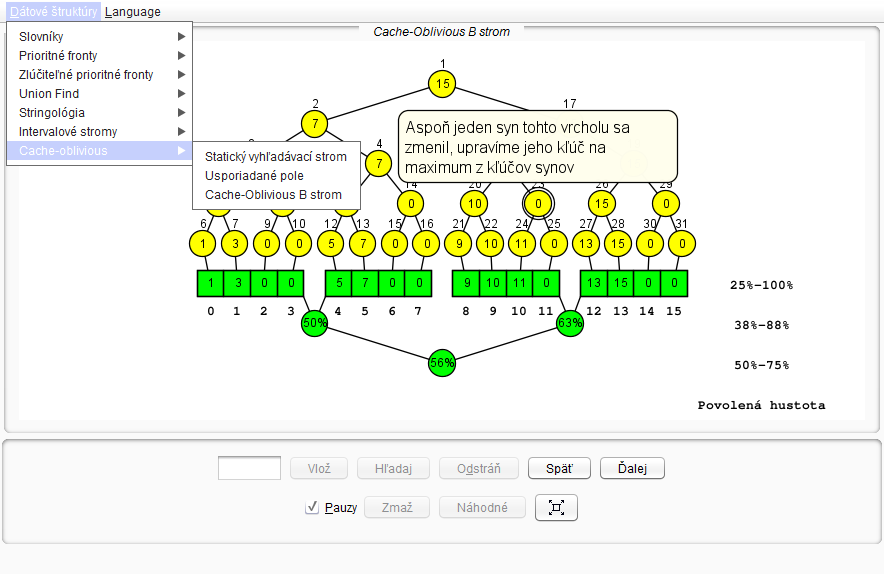
\includegraphics[width=18cm]{\FiguresPath/screenshots/bmp_cobtree_menu_sk}};
\draw [thick, darkgray] (IMG.south west) rectangle (IMG.north east);

%\draw[draw=red,xstep=1,ystep=1] (0,0) grid (18,12);
%\foreach \x in {0,1,...,18} { \node [anchor=north] at (\x,0) {\x}; }
%\foreach \y in {0,1,...,12} { \node [anchor=east] at (0,\y) {\y}; }

\draw [thick, ->] (2, 12.5) node [anchor=west] {Výber dátovej štruktúry} to [in=90, out=180] (1, 11.75);
\draw [thick, ->] (3, 12) node [anchor=west] {Výber jazyka} to [in=90, out=180] (2.5, 11.75);

\draw [thick, ->] (10, 12.5) node [anchor=west] {Aktuálna dátová štruktúra} to [in=90, out=180] (9, 11.25);

\draw [thick, ->] (13, 12) node [anchor=west] {Popis vykonávanej akcie} to [in=90, out=180] (11, 9.5);

\draw [thick, decoration={brace, amplitude=10pt, 
	/tikz/postaction = {
		decoration = {
			markings,
			mark = at position 0.5 with \coordinate (CP);
		}, decorate
	}
}, decorate] (4.25, 1) -- (4.25, 2.5);
\draw [thick] (2.5, -0.5) node [anchor=east] {Ovládací panel} to [in=180, out=0](CP);

\draw [thick, ->] (7, -0.5) node [anchor=west] {Povolenie krokovania} to [in=270, out=180] (6.35, 1.15);

\draw [thick, decoration={brace, amplitude=10pt, mirror,
	/tikz/postaction = {
		decoration = {
			markings,
			mark = at position 0.5 with \coordinate (PN);
		}, decorate
	}
}, decorate] (10.65, 1.95) -- (13.7, 1.95);
\draw [thick] (13, -0.5) node [anchor=west] {Krokovanie dopredu / dozadu} to [in=270, out=180] (PN);

\end{tikzpicture}    
    }
    \caption[Užívateľské rozhranie]{Užívateľské rozhranie počas operácie vkladania kľúča $10$ do dynamického \obliv B-stromu (sekcia \ref{sec:dynamic-obliv}).}
    \label{fig:ss_overview}
\end{figure}

Program sa skladá z troch hlavných častí (obrázok \ref{fig:ss_overview}). Najvrchnejšia časť okna tvorí hlavné menu, v ktorej môžeme voliť dátové štruktúry a prepínať jazyk rozhrania. Dátové štruktúry sú pre prehľadnosť rozdelené do niekoľkých kategórií. Tie popísané a implementované v tejto práci sa nachádzajú v kategórii \texttt{Cache-oblivious}.

V spodnej časti okna sa nachádza ovládací panel, ktorý obsahuje vstupné pole pre hodnotu, ktorú chceme vyhľadať alebo vložiť a tlačidlá na vykonanie týchto akcií. Ďalej obsahuje tlačidlá na prechod do ďalšieho kroku a návrat do predchádzajúceho stavu s možnosťou toto krokovanie vypnúť.

Najväčšia, prostredná časť okna zobrazuje vizualizáciu aktuálnej dátovej štruktúry. Toto zobrazenie je vektorové a je možné ho posúvať, približovať a oddaľovať. Zároveň sa tu zobrazujú informácie o aktuálne vykonávanej akcií (ak je povolené krokovanie) a ďalšie vizualizačné prvky ako šípky alebo význačné vrcholy.

Podrobnejší popis užívateľského rozhrania a návod na používanie sa nachádza v bakalárskej práci Jakuba Kováča \citep{algviskuko} v siedmej kapitole.

\section{Statický strom}
Najjednoduchšou dátovou štruktúrou je statický vyhľadávací strom. Implementovali sme vytvorenie tohto stromu a jeho uloženie v pamäti. Je možné strom zväčšiť alebo zmenšiť podľa preferencii - ukážky stromov rôznych veľkostí sú na obrázku \ref{fig:ss_static_sizes}. Čísla vo vnútorných vrcholoch sú kľúče, čísla nad vrcholom určujú jeho pozíciu v pamäti. Obdĺžnik nad stromom reprezentuje uloženie tohto stromu v poli. Vnútorné čísla sú opäť kľúče, pričom sú zoradené podľa svojich pozícii zľava (pozícia $1$) doprava.

\begin{figure}
    \centering
    \subtop[]{%
        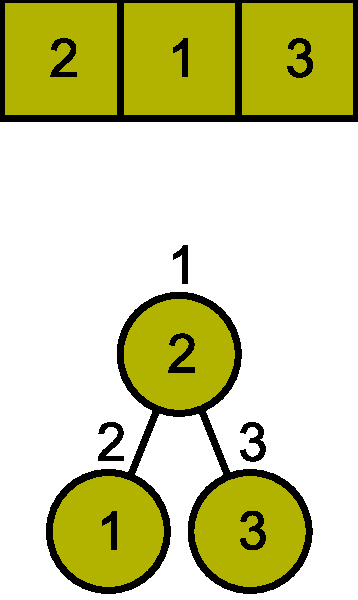
\includegraphics[scale=0.25]{figures/screenshots/static_size_2.pdf}}
    \hspace{0.5cm}
    \subtop[]{%
        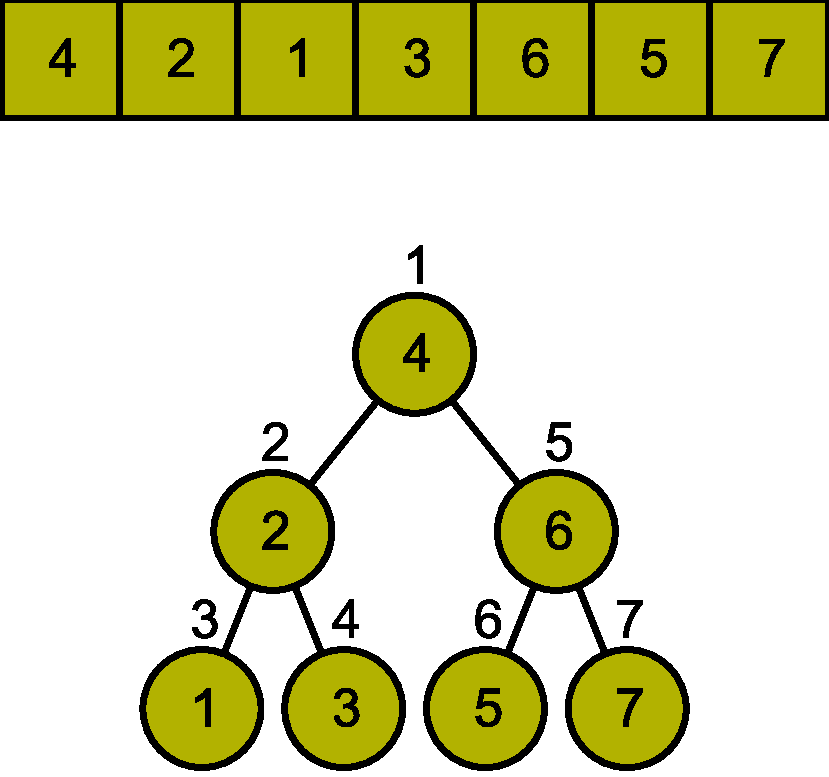
\includegraphics[scale=0.25]{figures/screenshots/static_size_3.pdf}}
    \hspace{0.5cm}
    \subtop[]{%
        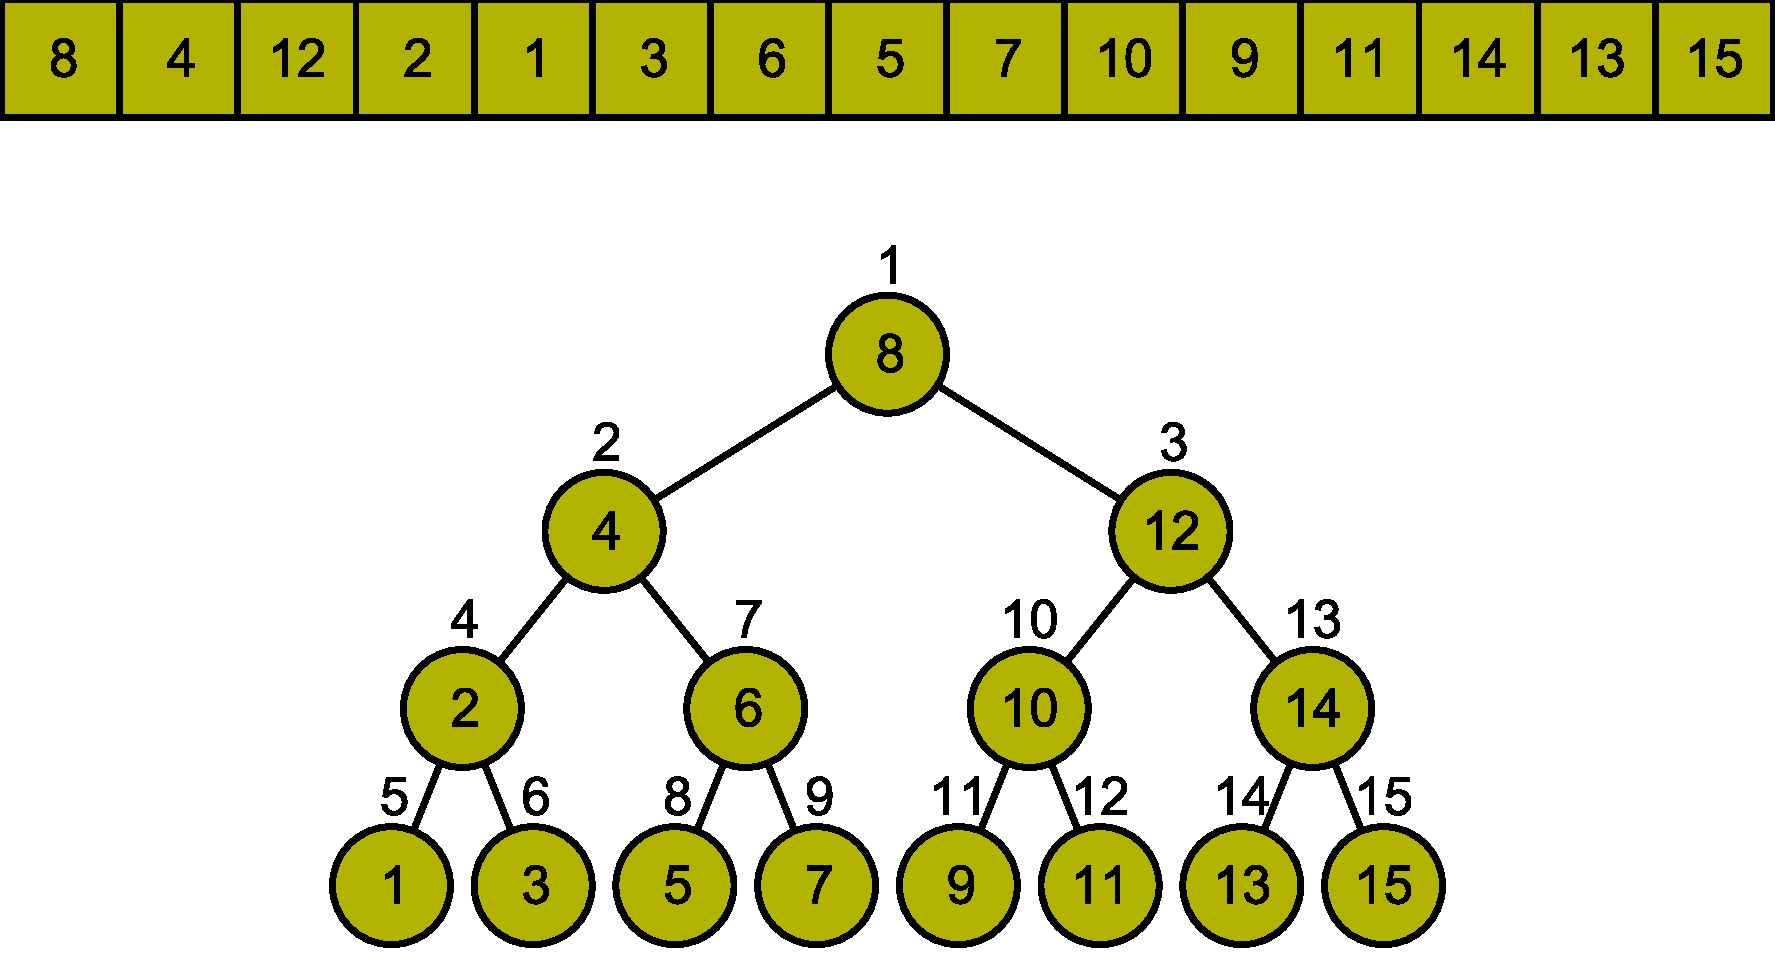
\includegraphics[scale=0.25]{figures/screenshots/static_size_4.pdf}}
    \caption[Statické stromy rôznych veľkostí]{Statické stromy rôznych veľkostí (výšok) vo \vEB usporiadaní.}
    \label{fig:ss_static_sizes}
\end{figure}

Medzi uložením vo \vEB usporiadaní a klasickom \emph{BFS} usporiadaní (ako v časti \ref{sec:static-naive}) je možné prepínať. Zmenia sa pritom čísla udávajúce pozície vrcholov v pamäti a ich poradie v poli nad stromom. Rozdiel medzi týmito dvoma usporiadaniami vidieť na obrázku \ref{fig:ss_static_order}. Pozície sa zhodujú s obrázkom \ref{fig:node_order_veb}.

\begin{figure}
    \centering
    \subtop[]{%
        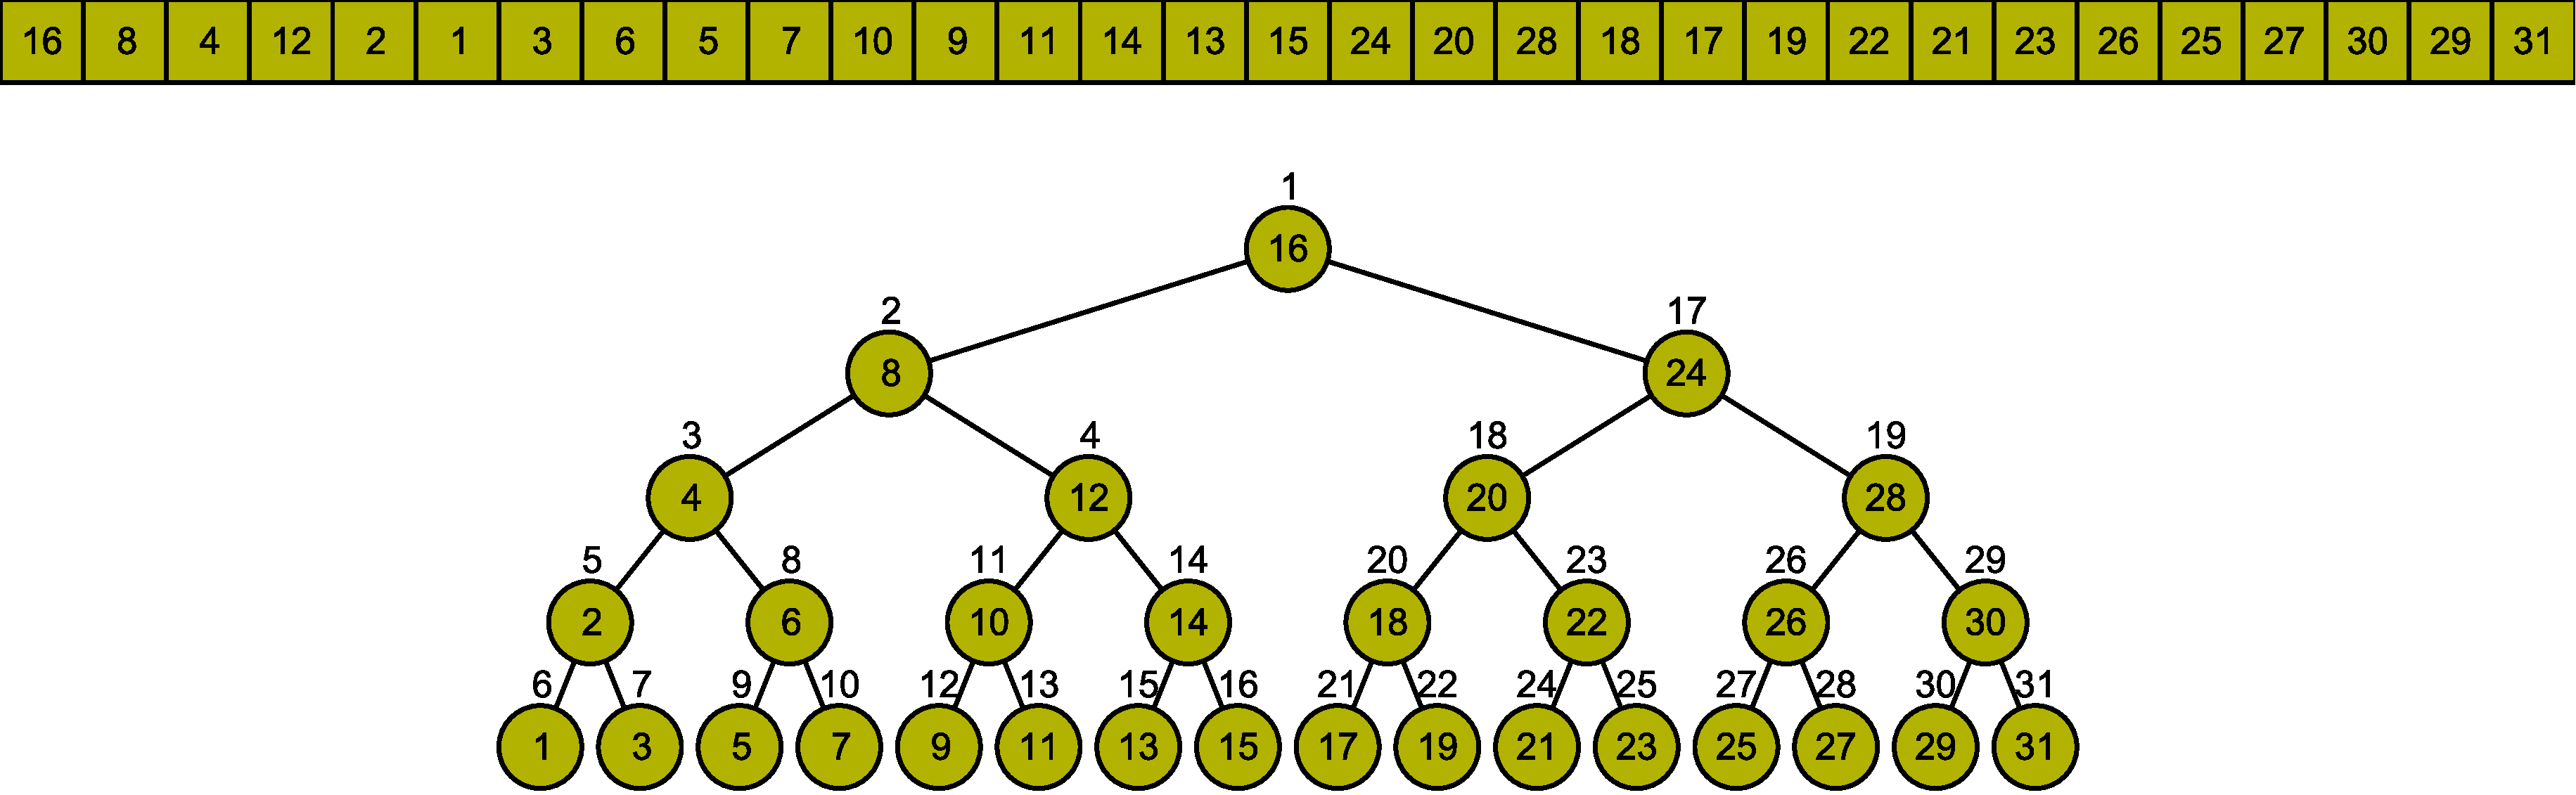
\includegraphics[width=\textwidth]{figures/screenshots/static_size_5.pdf}}
    \subtop[]{%
        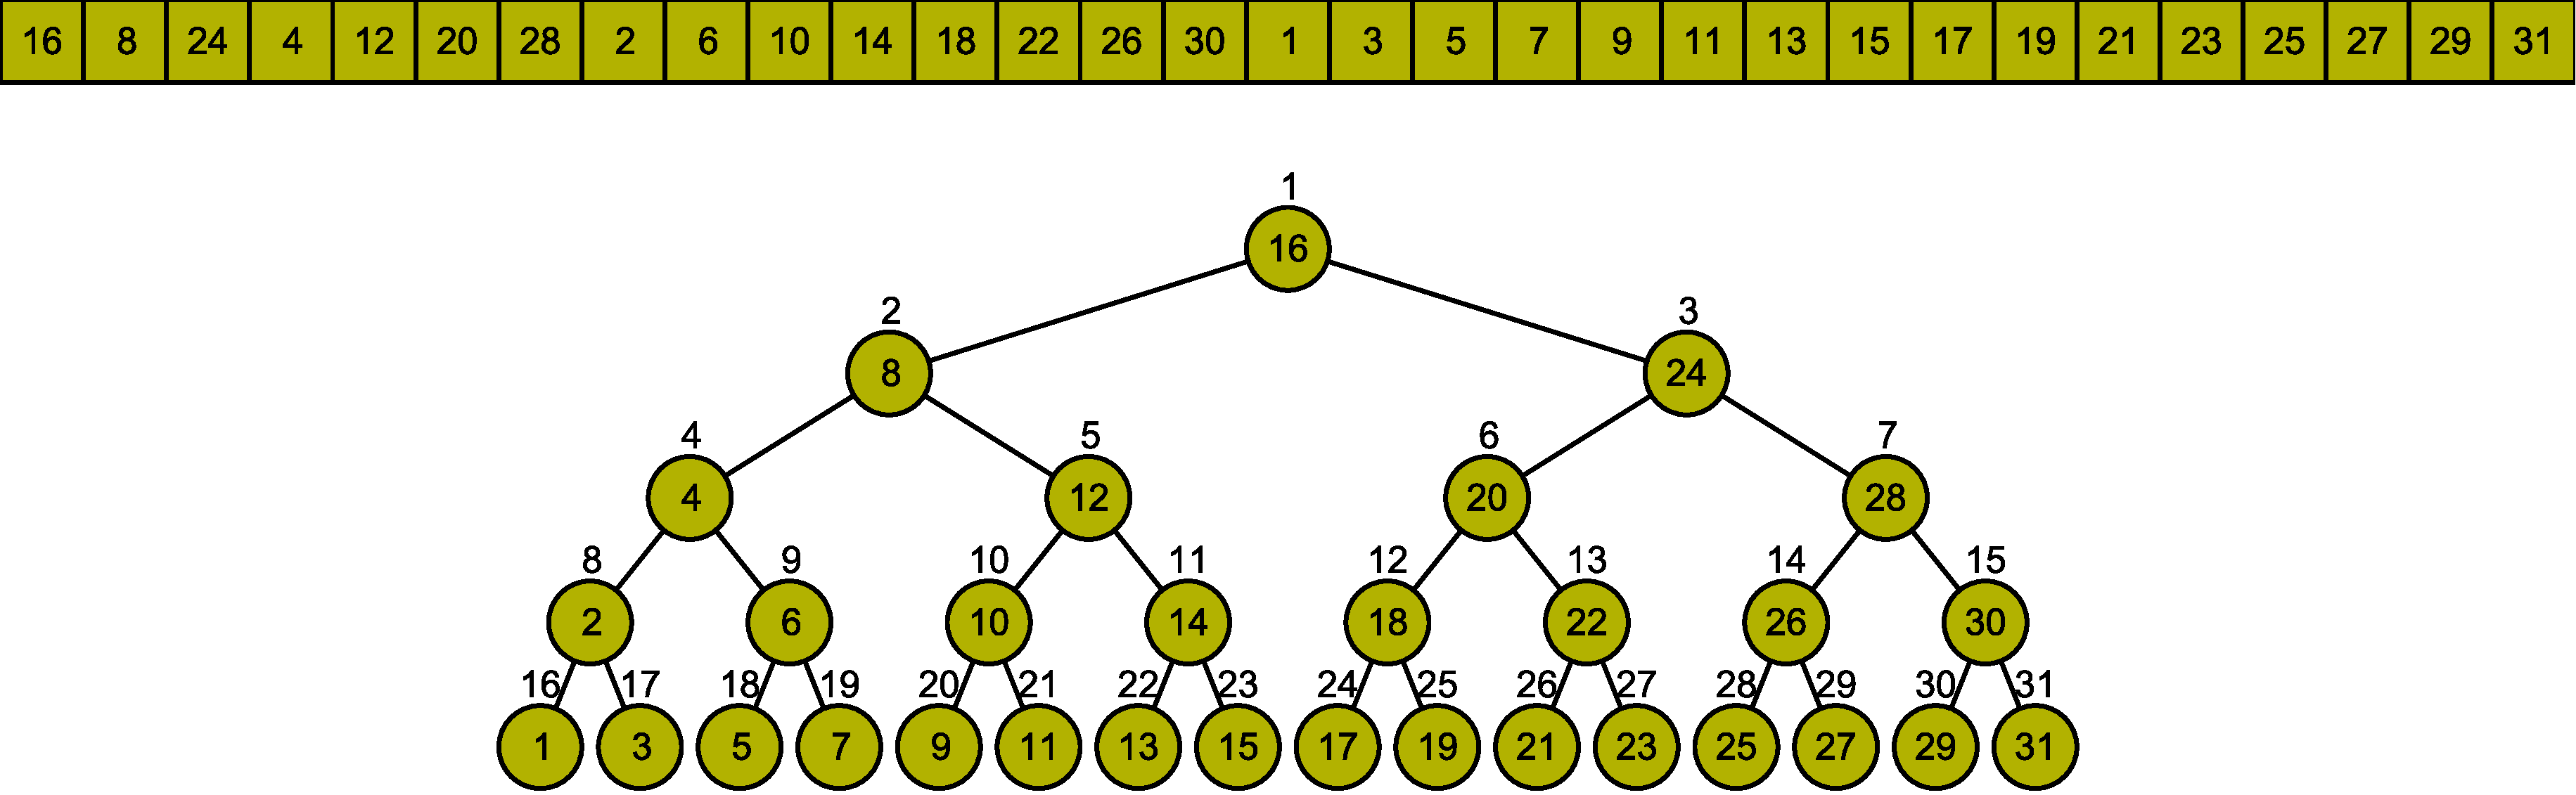
\includegraphics[width=\textwidth]{figures/screenshots/static_size_5_bfs.pdf}}
    \caption[Rozdiel medzi \emph{BFS} a \vEB usporiadaním]{Rozdiel medzi \emph{BFS} a \vEB usporiadaním na strome výšky~$5$. Kľúče zostávajú rovnaké, líšia sa však ich pozície v pamäti reprezentované malými číslami nad vrcholmi a poľom nad koreňom.}
    \label{fig:ss_static_order}
\end{figure}

\subsection{Simulácia \cache}
Porovnanie týchto dvoch usporiadaní je rozšírené o simuláciu \cache. Užívateľ si môže zvoliť parametre cache - počet vrcholov $B$, ktoré sa zmestia do jedného bloku a počet blokov $\frac{M}{B}$ v \cache. Tiež je možné \cache kedykoľvek vyprázdniť -- odstrániť z nej všetky načítané bloky. Simulácia na výmenu stránok používa stratégiu \emph{FIFO}, ktorá je popísaná v časti \ref{sec:memmng}.

Táto simulácia zároveň počíta počet prístupov k vrcholom pri vyhľadávaní a počet presunutých blokov do \cache. V najhoršom prípade by tieto dve čísla boli rovnaké (ak treba každý vrchol načítať osobitne) avšak pri \cache s blokmi veľkosti $B > 1$ a s \vEB usporiadaním dochádza k podstatnému zlepšeniu - ušetreniu počtu presunutých blokov.

To môžeme vidieť na jednoduchom príklade, kedy v strome výšky $5$ postupne vyhľadáme všetkých $16$ kľúčov, ktoré sa nachádzajú v listoch tohto stromu. V oboch usporiadaniach bude počet prístupov rovnaký, avšak počet načítaní blokov z disku do \cache je v tomto príklade pri \emph{BFS} usporiadaní takmer dvakrát väčší ako pri \vEB usporiadaní. Obrázok \ref{fig:ss_cachesim_compare} ukazuje stav týchto štatistík po nájdení posledného listu.

\begin{figure}[h]
    \centering
    \subbottom[Strom v \emph{BFS} usporiadaní] {
        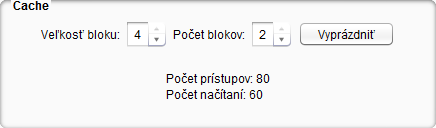
\includegraphics[width=6cm]{figures/screenshots/bmp_cache_panel_leaves_bfs}
    }
    \hspace{1cm}
    \subbottom[Strom vo \vEB usporiadaní] {
        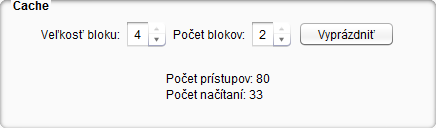
\includegraphics[width=6cm]{figures/screenshots/bmp_cache_panel_leaves_veb}
    }
    \caption[Porovnanie štatistík simulovanej \cache]{Porovnanie štatistík simulovanej \cache po prechode listov $1,3,\dotsc,31$ stromu výšky $5$. Parametre cache sú v oboch prípadoch rovnaké ($B=4$, $M=2B=8$), rozdiel je však v usporiadaní v pamäti.}
    \label{fig:ss_cachesim_compare}
\end{figure}

Ako vizualizácia prítomnosti v \cache slúži farba - vrcholy a položky poľa obsahujúce kľúče majú svetlejšiu farbu pozadia v prípade, že je daný blok v \cache a tmavšiu ak je mimo. V strome je vďaka tomu ľahko vidieť, ktorá časť je načítaná a je možné ňou prechádzať bez ďalších presunov. V prípade \vEB usporiadanie pôjde prevažne o časť podstromu aktuálne porovnávaného vrcholu, avšak pri klasickom usporiadaní to budú práve vrcholy mimo tohto podstromu, o ktorých už vieme, že nie sú pri vyhľadávaní potrebné.

\begin{figure}
    \centering
    \subtop[Nultý krok]{%
        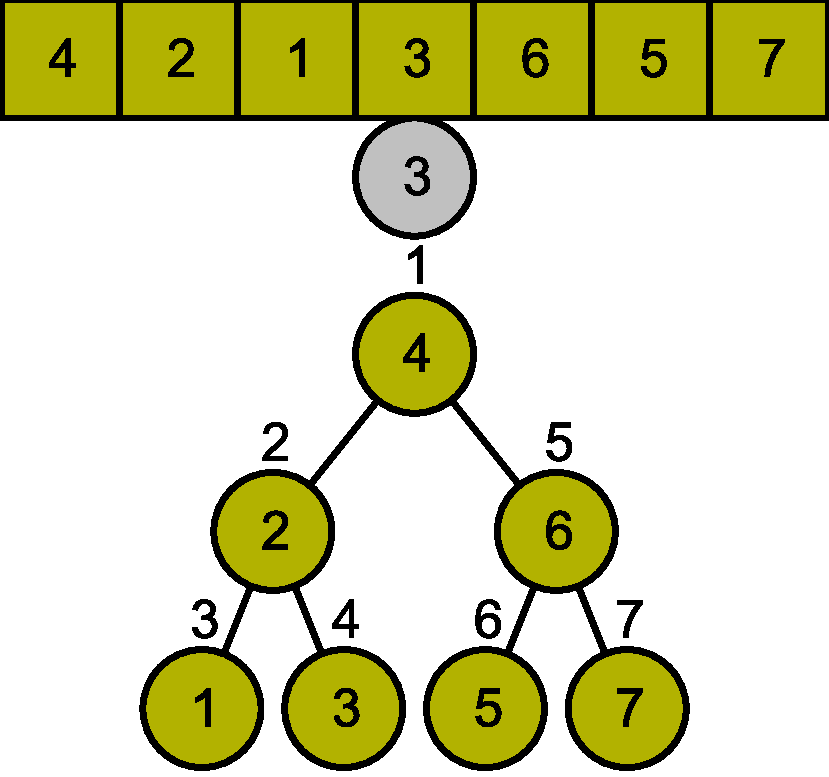
\includegraphics[width=0.25\textwidth]{figures/screenshots/cachesim_step1.pdf}}
    \hspace{1cm}
    \subtop[Prvý krok]{%
        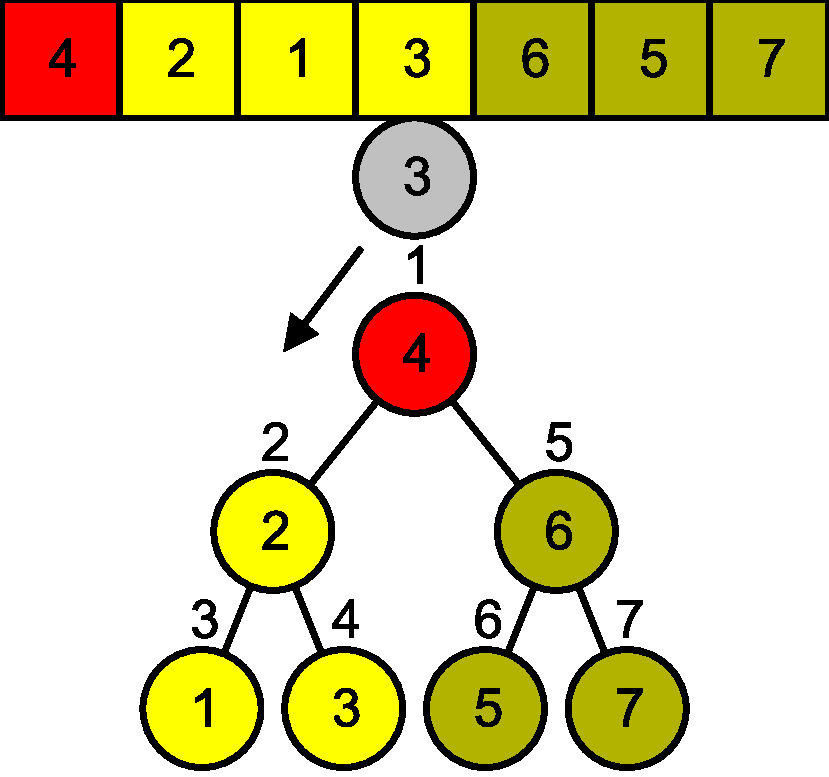
\includegraphics[width=0.25\textwidth]{figures/screenshots/cachesim_step2.pdf}}
    \hspace{1cm}
    \subtop[Druhý krok]{%
        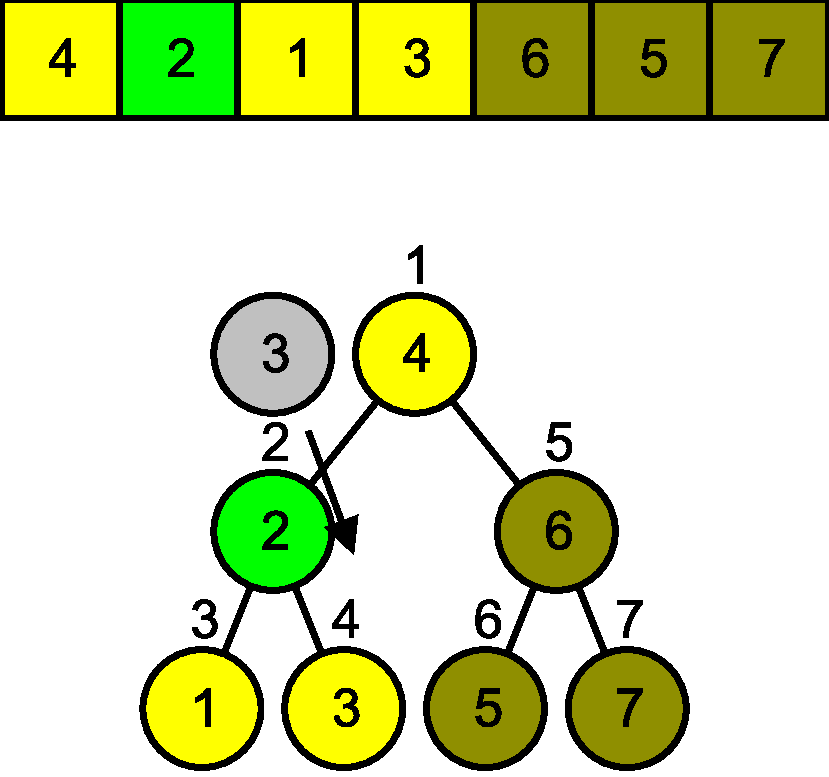
\includegraphics[width=0.25\textwidth]{figures/screenshots/cachesim_step3.pdf}}
    \caption[Simulácia \cache počas vyhľadávania kľúča]{Simulácia \cache počas vyhľadávania kľúča $3$. Pred prvým prístupom je cache prázdna. V prvok kroku načítame koreň, ktorý je označený červenou farbou (\miss), keďže nebol v \cache. Spolu s ním sa v jednom bloku načítali ďalšie vrcholy, ktoré su označené svetlejšou farbou. V druhom kroku je vrchol s kľúčom $2$ označený zelenou farbou (\hit), keďže už bol do \cache načítaný v predchádzajúcom kroku.}
    \label{fig:ss_cachesim_colors}
\end{figure}

Pri krokovaní vyhľadávania je pri prístupe k vrcholu tiež použitá zelená alebo červená farba na jeho dočasné zafarbenie (podobne ako v časti \ref{sec:memaccess_patterns}) podľa toho, či sa v danom momente v \cache nachádzal (\hit) alebo nie (\miss). Ukážka tohto zafarbovania je na obrázku \ref{fig:ss_cachesim_colors}.

\section{Usporiadané pole}
Ďalšou implementovanou vizualizáciou je usporiadané pole (obrázok \ref{fig:ss_of_overview}), ktoré bolo popísané v časti \ref{sec:orderedfile}. Bloky, na ktoré je toto pole imaginárne rozdelené sú znázornené tým, že sú od seba oddelené medzerou. Taktiež sa zobrazuje imaginárny strom nad týmito blokmi, ktorým sa pri vkladaní prechádza. Hodnoty vo vrcholoch reprezentujú hustotu (v percentách) intervalu v príslušnom podstrome. Farby (zelená alebo červená) vrcholov indikujú, či sa hustota daného vrcholu nachádza v hraniciach.

\begin{figure}
    \centering
    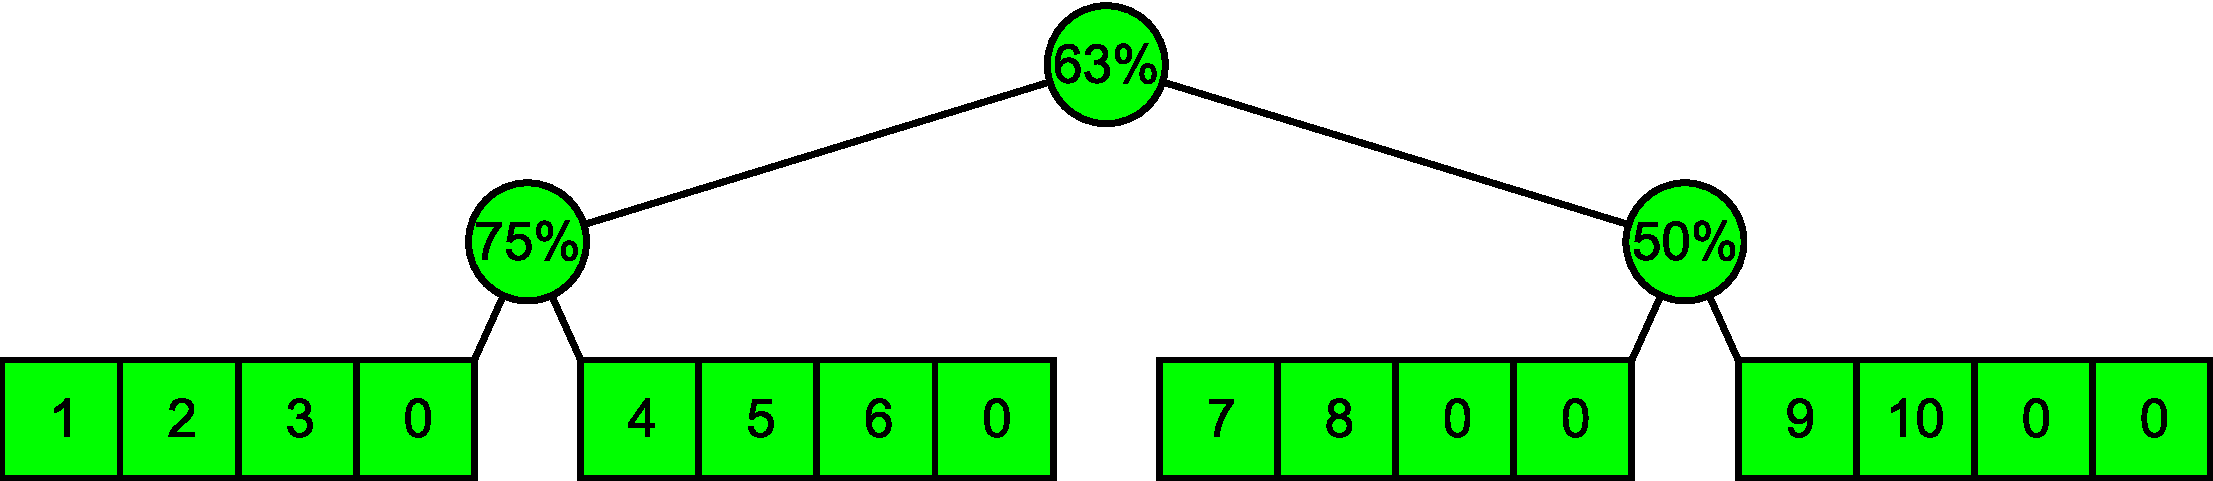
\includegraphics[width=0.8\textwidth]{figures/screenshots/of_overview_3.pdf}
    \caption[Usporiadané pole]{Usporiadané pole obsahujúce hodnoty $1$ až $10$. Všetky vrcholu majú hustotu v hraniach hustoty. Hodnoty $0$ reprezentujú prázdne pozície.}
    \label{fig:ss_of_overview}
\end{figure}

Táto vizualizácia podporuje vkladanie hodnoty na ľubovolnú pozíciu v poli. V prípade, že sa pole preplní, automaticky sa vytvorí nové, dvojnásobne väčšie. Po vložení hodnoty je tiež vyznačený interval, ktorý sa zmenil.

\section{Dynamický strom}
Vizualizácia dynamického stromu (časť \ref{sec:dynamic-obliv}) vznikla spojením predchádzajúcich dvoch vizualizácií (obrázok \ref{fig:ss_cobtree}). Horná časť je statický strom vo \vEB usporiadaní (obrázok \ref{fig:ss_static_sizes}), dolná je usporiadané pole (obrázok \ref{fig:ss_of_overview}), pričom strom hustôt je tu preklopený nadol, aby sa neprekrýval so statickým stromom. Hrany medzi nimi spájajú listy stromu s prvkami usporiadaného pola. 

\begin{figure}
    \centering
    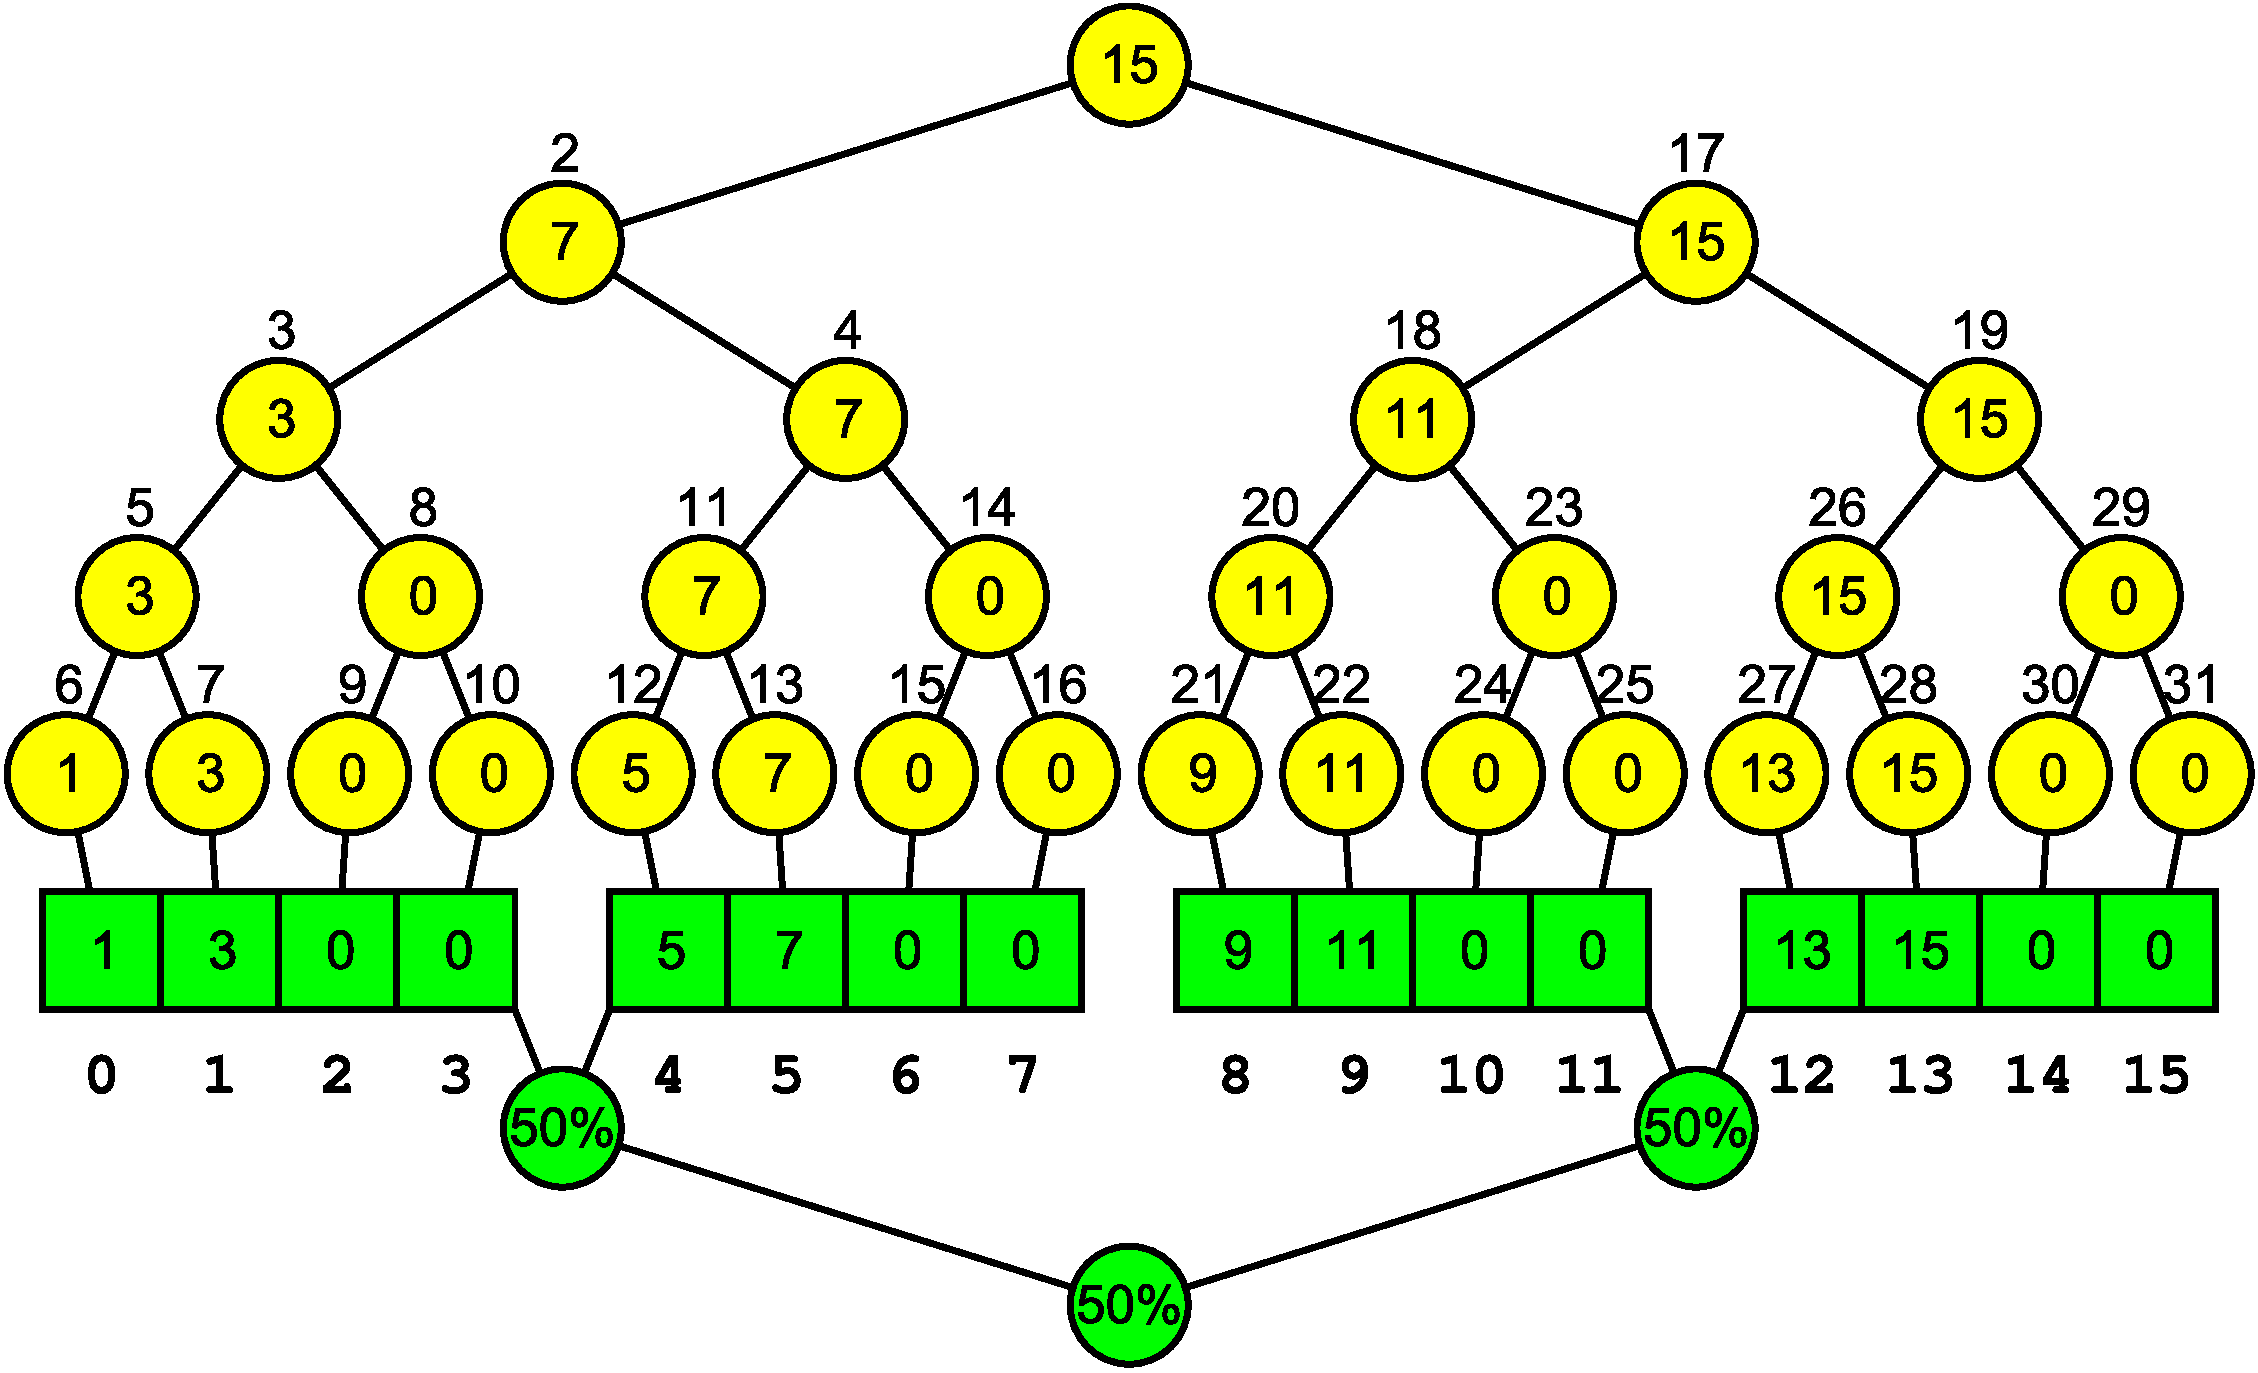
\includegraphics[width=0.8\textwidth]{figures/screenshots/cobtree_overview.pdf}
    \caption[Vizualizácia dynamického \obliv B-stromu]{Vizualizácia dynamického \obliv B-stromu.}
    \label{fig:ss_cobtree}
\end{figure}

V tomto strome je možné vyhľadávať a vkladať do neho nové kľúče. Pri vkladaní prebehne najskôr vloženie do usporiadaného poľa rovnako, ako pri jeho samostatnej vizualizácii. Následne sa aktualizujú kľúče statického stromu. V prípade zdvojnásobenia veľkosti statického poľa sa vytvorí nový, väčší statický strom.


\section{Implementácia}
\todo[inline]{?}

%Visualization
%- intro
%- existing - none?
%- algvis history
%- implementation details
%  - cache simulation
%- list of structures
%  - static tree
%    - intro
%    - array order
%    - cache simulation
%    - order switching
%  - ordered file
%    - intro
%    - insert
%  - cobtree
%    - intro
%    - layout
%    - find
%    - insert
%- testovanie?


\backmatter
    \nocite{*} % Add all bibliography uncited in text
    \bibliography{research}
    
    \clearpage
\pagestyle{empty}
\null\vfil

\begin{adjustwidth}{2cm}{2cm}
\begin{center}
{\Large\textsf{Kolofón}}
\end{center}
\noindent Sadzba tejto práce bola vykonaná systémom \textsf{\XeLaTeX} s použitím šablóny \textsf{memoir}. Literatúra bola spravovaná systémom \textsf{\BibTeX}. Ilustrácie sú vyrobené pomocou balíčkov \textsf{Ti\textit{k}Z/PGF}.

\vspace{1cm}

\begin{center}
{\Large \ccbyncndeu}
\end{center}

\noindent Text tejto práce je zverejnený pod \textsf{Creative Commons} licenciou verzie \textsf{BY-NC-ND 3.0}, ktorej plné znenie sa nachádza na stránke \url{https://creativecommons.org/licenses/by-nc-nd/3.0/}.

\vspace{1cm}

\noindent Zdrojový text tejto práce spolu so všetkými ilustráciami je dostupný na stránke \url{https://github.com/lacop/thesis}.

\end{adjustwidth}

\vfil
\end{document}
